%%%%%%%%%%%%%%%%%%%%%%%%%%%%%%%%%%%%%%%%%
% Thin Sectioned Essay
% LaTeX Template
% Version 1.0 (3/8/13)
%
% This template is based on a downloaded from:
% http://www.LaTeXTemplates.com
%
% Original Author:
% Nicolas Diaz (nsdiaz@uc.cl) with extensive modifications by:
% Vel (vel@latextemplates.com)
% and adjustments by 
% Thuy Tran 
%
% License:
% CC BY-NC-SA 3.0 (http://creativecommons.org/licenses/by-nc-sa/3.0/)
%
%%%%%%%%%%%%%%%%%%%%%%%%%%%%%%%%%%%%%%%%%

%----------------------------------------------------------------------------------------
%	PACKAGES AND OTHER DOCUMENT CONFIGURATIONS
%----------------------------------------------------------------------------------------

\documentclass[a4paper, 12pt]{report} % Font size (can be 10pt, 11pt or 12pt) and paper size (remove a4paper for US letter paper)

\usepackage[protrusion=true,expansion=true]{microtype} % Better typography
\usepackage{graphicx} % Required for including pictures
\usepackage{wrapfig} % Allows in-line images
\usepackage{listings}
\usepackage{mathpazo} % Use the Palatino font
\usepackage[T1]{fontenc} % Required for accented characters
\usepackage[utf8]{inputenc} 
\usepackage[ngerman]{babel}
\linespread{1.05} % Change line spacing here, Palatino benefits from a slight increase by default
\usepackage{hyperref} %To include URLs
\usepackage{caption}
\usepackage{adjustbox}
\usepackage{placeins}


\makeatletter
\renewcommand\@biblabel[1]{\textbf{#1.}} % Change the square brackets for each bibliography item from '[1]' to '1.'
\renewcommand{\@listI}{\itemsep=0pt} % Reduce the space between items in the itemize and enumerate environments and the bibliography

\renewcommand{\maketitle}{ % Customize the title - do not edit title and author name here, see the TITLE block below
\begin{center} % Right align
{\LARGE\@title} % Increase the font size of the title

\vspace{50pt} % Some vertical space between the title and author name

{\large\@author} % Author name
\vspace{10pt}
\\\@date % Date

\vspace{40pt} % Some vertical space between the author block and abstract
\end{center}
}

%----------------------------------------------------------------------------------------
%	TITLE
%----------------------------------------------------------------------------------------
%\begingroup
\vspace{1.5cm}
\title{\textbf{}\\ % Title
Erstellung einer Schnittelle zwischen \\ einem Anonymiserungstool f{\"u}r \\ medizinische Daten und dem \\ Statistikprogramm R\\} % Subtitle

%\endgroup

\author{
\textsc{Klinisches Anwendungsprojekt}
\vspace{15pt}
\\ \textit{Institut für Medizinische Statistik und Epidemiologie, 
\\Klinikum rechts der Isar der TUM} % Institution
\vspace{10pt}
\\ \textit{Bearbeiter: Alexander Beischl und Thuy Tran} % Author
\vspace{10pt}
\\ \textit{Aufgabensteller: Prof. Dr. Klaus A. Kuhn} 
\vspace{10pt}
\\ \textit{Betreuer: Dr. Fabian Prasser}}

\date{\today} % Date

%----------------------------------------------------------------------------------------

\begin{document}
\renewcommand\lstlistingname{R-Befehl}

\maketitle % Print the title section

%----------------------------------------------------------------------------------------
%	ABSTRACT AND KEYWORDS
%----------------------------------------------------------------------------------------

\renewcommand{\abstractname}{Zusammenfassung} % Uncomment to change the name of the abstract to something else

\begin{abstract}

\noindent
Zum Schutz von medizinischen Daten bietet sich die Möglichkeit der  Datenanonymisierung an. Hierbei soll eine Veränderung der Daten die Beziehung zwischen den Daten und den Datensubjekten verschleiern. 

Bei der Verwendung des Datenanonymisierungstools \textit{ARX} kommt es bei jeder Anonymisierung zu einem Informationsverlust und Verzerrungen der statistischen Eigenschaften. 
Um dabei die Auswirkungen der Anonymisierung auf eine Vielzahl statistischer Eigenschaften und Verfahren analysieren zu können, bietet sich die Nutzung eines Statistikprogramms wie \textit{R} an.
Allerdings ist eine Integration von \textit{R} in \textit{ARX} aufgrund von Lizenzrechten nicht möglich. 

Aus diesem Grund wurde im Rahmen des Klinisches Anwendungsprojektes die \textit{Java}-Software \textit{R-Terminal} implementiert, welches im Rahmen dieser Ausarbeitung vorgestellt wird. Dieses Programm integriert \textit{R} in \textit{Java}, sodass \textit{R}-Befehle und \textit{R}-Skripte in \textit{Java} ausgeführt werden können. Hierfür wird durch das \textit{R-Terminal} eine Standalone-Installation von \textit{R} durch \textit{ProcessBuilder} als Prozess gestartet und die Kommunikation mittels Input- und Output-Stream hergestellt.

Das \textit{R-Terminal} verfügt über eine optionale graphische Benutzeroberfläche. 
Mit dem \textit{R-Terminal} können außerdem auf Datensätzen, welche aus dem  Anonymisierungs-Tool \textit{ARX} exportiert wurden, \textit{R}-Befehle ausgeführt werden. 
\end{abstract}


\vspace{30pt} % Some vertical space between the abstract and first section
%----------------------------------------------------------------------------------------

\tableofcontents


%----------------------------------------------------------------------------------------
%	ESSAY BODY
%----------------------------------------------------------------------------------------

\chapter{Einleitung}\label{einführung}

Der Austausch von sensiblen personenbezogenen Daten spielt in der modernen medizinischen Forschung eine wichtige Rolle. Hierbei muss die Privatsphäre der betroffenen Patienten oder Probanden geschützt werden. Eine Möglichkeit dazu ist die Datenanonymisierung. Anonymisierung meint in diesem Zusammenhang die Veränderung personenbezogener Daten derart, dass die Beziehung zwischen den Daten und den Datensubjekten nur mit unverhältnismäßigem Aufwand wiederhergestellt werden kann.
Hierfür wurde das Datenanonymisierungstool \textit{ARX} vom Institut für Medizinische Statistik und Epidemiologie der Technischen Universität München entwickelt, welches verschiedene Methoden der Datenanonymisierung implementiert.

Diese Notwendigkeit zur Wahrung der Privatsphäre der Patienten führt allerdings auch zu Informationsverlust und einer Verzerrung statistischer Eigenschaften. Die Anonymisierung eines Datensatzes kann somit dazu führen, dass dieser unter Umständen nicht mehr nutzbar ist. Deshalb müssen außerdem untersucht werden können, ob die Daten weiterhin für den geplanten Forschungszweck verwendbar sind. Hierfür ist es hilfreich, mithilfe von statistischen Funktionen die Auswirkung der Anonymisierung auf einen solchen Datensatz überprüfen zu können. 

 Obwohl \textit{ARX} bereits grundlegenden statistischen Methoden zur Analyse bereitstellt, bietet es sich an, die Programmiersprache und Entwicklungsumgebung \textit{R} zu verwenden, um mit den anonymisierten Patientendaten aus \textit{ARX} zu arbeiten und statistische Analysen durchzuführen.
 \textit{R} bietet als spezialisierte Statistiksoftware eine umfangreiche Sammlung an Funktionen zur statistischen Auswertung von Daten an und ist ein wichtiges Werkzeug für Statistikanalysen der medizinischen Forschung.  

Zusätzlich kann das \textit{R}-Paket \textit{sdcMicro} verwendet werden, welches sowohl Funktionen zur Anonymisierung, als auch Methoden zur Risikoeinschätzung von Anonymisierung bereitstellt \cite{sdc}. Dadurch können Datensätze direkt in \textit{R} anonymisiert und statistisch untersucht werden, wodurch potenzielle Abweichungen ausfindig gemacht werden können. 

Durch die Verwendung von \textit{R} sollen somit die Ein- und anonymisierte Ausgabe der Patientendaten aus \textit{ARX} untersucht werden, um die statistischen Abweichungen zu analysieren und die Verwendbarkeit der anonymisierten Daten zu untersuchen.
 
\subsection*{Möglichkeiten der Integration}

Eine Verlinkung auf \textit{R} ist aus \textit{ARX} aufgrund der jeweiligen Lizenzierung leider nicht möglich, was nicht technische, sondern rechtliche Gründe hat.

\textit{ARX} ist unter der Apache License lizensiert, während \textit{R} als GNU-Projekt unter GPL (GNU General Public License) lizensiert ist. 
Obwohl beide Lizenzen für freie Software genutzt werden, welche den Nutzern kaum Restriktionen im Umgang mit der Software auferlegen, sind sie nicht miteinander kompatibel. Während Software unter Apache License in GPL Projekten integriert werden dürfen, lässt GPL umgekehrt dies nicht zu. 

Diese Inkompatibilität kommt zustande, wenn Software unter Apache mit von GPL Software abgeleiteten Projekten geschrieben wird. Dadurch muss diese unter GPL gestellt werden. In diesem Falle müsste \textit{ARX} als Apache License Projekt unter GPL gestellt werden, um es gemeinsam mit \textit{R} zu verwenden. Dies wiederum lässt die Apache License nicht zu, da jede Apache Software unter Apache lizensiert werden muss. Es ist weitgehend von GPL-Autoren interpretationsbedingt, was ein von GPL Software abgeleitetes Projekt ist. Um hierbei Komplikationen zu vermeiden, ist es nicht ratsam, von aus Apache Software GPL Software zu verlinken \cite{license}. 

Das Ziel des in diesem Rahmen entwickelten \textit{RTerminals} ist es, eine Möglichkeit zur Verfügung zu stellen \textit{R} aufzurufen, innerhalb des \textit{RTerminals} \textit{ARX}-Daten einzulesen und diese zu bearbeiten.

Das \textit{RTerminal} bietet hierfür eine Schnittstelle um \textit{R} in einer eigenen GUI auszuführen und \textit{ARX}-Daten einzulesen sowie zu bearbeiten. Zusätzlich soll es Funktionen bieten, die eine dynamische Arbeit mit \textit{R} erleichtern.
Es existieren zwar bereits für \textit{Java} Pakete wie \textit{RServe}, \textit{JRI} und \textit{RCaller}, welche ebenfalls eine Integration realisieren, eine direkten Nutzung von JRI und RCaller mit \textit{ARX} ist aufgrund der jeweiligen Lizenzierung aber nicht möglich.

Der TCP/IP-Server \textit{RServe} erlaubt es eine Verbindung zu \textit{R} aufzubauen, ohne \textit{R} initialisieren oder aufrufen zu müssen. Damit wäre es kein lizenzrechtliches Problem, \textit{RServe} zu verwenden. 

Allerdings ist es umständlich, einen Webserver zu installieren, weswegen \textit{RServe} sich nicht als leichtgewichtige Option zur \textit{R}-GUI
anbietet. 

Aus diesem Grund wurde für das \textit{RTerminal} die Integration von \textit{R} als leichtgewichtiger Subprozess gewählt, bei welchem die Kommunikation zwischen dem \textit{RTerminal} und dem \textit{R}-Prozess über den Standardinput und Standardoutput des \textit{R}-Prozesses erfolgt.\\
\\
In dieser Ausarbeitung werden in dem Kapitel "`Design und Implementierung"' die technischen Hintergründe des \textit{RTerminals} erläutert und die Klassen der Implementierung dokumentiert.
Die Benutzung sowie die Features des \textit{RTerminals} werden unter "`Ergebnis"' vorgestellt.
Im Kapitel "`Benutzung von R für ARX"' werden Möglichkeiten für den Import von n aus \textit{ARX} in \textit{R} vorgestellt, welche allerdings noch nicht implementiert wurden.
Das letzte Kapitel beinhaltet die wichtigsten Funktionen, welche in zukünftigen Arbeiten implementiert werden sollen.

%------------------------------------------------

%\section*{R}\label{r}
%R ist eine Programmiersprache und Entwicklungsumgebung, die für statistische Berechnungen und Graphen unter John Chambers von Bell Laboratories entwickelt wurde. Sie ist ein \textit{GNU}-Projekt, bei dem die Entwicklung von freier Software im Mittelpunkt steht. \textit{R} weist große Ähnlichkeiten zu der Programmiersprache \textit{S} auf, einem weiteren \textit{GNU}-Projekt, welches weitgehend auch unter \textit{R} läuft. \cite{rproject}

%\textit{R} bietet standardmäßig alle Hauptfunktionen für die statistische Analyse von Datensätzen an und ist einfach zu erweitern, weswegen es vor allem für wissenschaftliche Arbeiten verwendet wird. Es ist mit \textit{R} einfach, statistische Funktionen auf große Datenmengen anzuwenden. \cite{rproject}


%------------------------------------------------

%\section*{ARX}
%\textit{ARX} ist eine freie Software zur Anonymisierung von medizinischen Datensätzen, die von Fabian Prasser und Florian Kohlmayer vom Institut für medizinische Statistik und Epidemiologie an der Technischen Universität München entwickelt wurde. \cite{arx}


%\section*{Vorgaben}

%Für die Implementierung der Software wurde \textit{Java} als Programmiersprache vorgegeben, außerdem sollte die graphische Benutzeroberfläche mit \textit{SWT} realisiert werden.

%Die graphische Benutzeroberfläche sollte aus unterschiedlichen Tabs aufgebaut sein. Ein Tab beinhaltet folgende Informationen zum Setup: verwendetes Betriebssystem, aktuell integrierte Version von \textit{R} und Installationsort der \textit{R}-Version. In einem weiteren Tab wird der Std-Output von \textit{R} ausgegeben und \textit{R}-Befehle können in diesem Tab eingegeben werden. 

%Beim Programmstart soll automatisch in den Standart-Installationsorten nach einer ausführbaren \textit{R}-Executive gesucht werden. Außerdem soll die Möglichkeit bestehen, manuell eine \textit{R}-Installation auszuwählen und diese mit der Software in \textit{Java} zu integrieren. 


\chapter{Design und Implementierung}

\section{Verwendete Technologien}

Das \textit{R-Terminal} wurde mit der Entwicklungsumgebung \textit{Eclipse} \cite{eclipse} entwickelt.
Als Programmiersprache wurde \textit{Java} \cite{java} gewählt. Die grafische Benutzeroberfläche wurde mit \textit{SWT} \cite{swt} realisiert, genauere Details hierzu werden in \ref{swt} erläutert.
Um \textit{R}-Kommandos auszuführen, startet das hier dokumentierte Programm \textit{R-Terminal} einen \textit{R}-Prozess der Standalone-Installation von \textit{R} durch die \textit{Java}-Library \textit{ProcessBuilder} \cite{processBuilder}.


\section{Architektur des R-Terminals}

Die Software des \textit{R-Terminal} ist in zwei Komponenten aufgeteilt, welche als getrennte Packages vorliegen. Das erste Package "`org.deidentifier.arx.gui"' beinhaltet die graphische Benutzeroberfläche, das Zweite "`org.deidentifier.arx.r"' beinhaltet die gesamte Integration von \textit{R} in \textit{Java}, es stellt also alle funktionalen Methoden zur Verfügung und verwaltet die Kommunikation zwischen \textit{R} und dem \textit{Java}-Programm.

Durch die Trennung von graphischer Benutzeroberfläche und der Integration von \textit{R}, also dem funktionalen Kern, kann die \textit{R}-Integration auch ohne graphische Benutzeroberfläche ausgeführt und verwendet werden. Hierzu wird nur das zweite Package benötigt, welches in \ref{funktionaler Kern} behandelt wird. Die Ausführung ohne GUI wird in \ref{ohne GUI} erläutert.\\

Alle Klassen der Software \textit{R-Terminal}, sowie deren wichtigsten Methoden, werden in den Kapiteln \ref{gui} und \ref{funktionaler Kern} vorgestellt.

\begin{figure}[h!]
		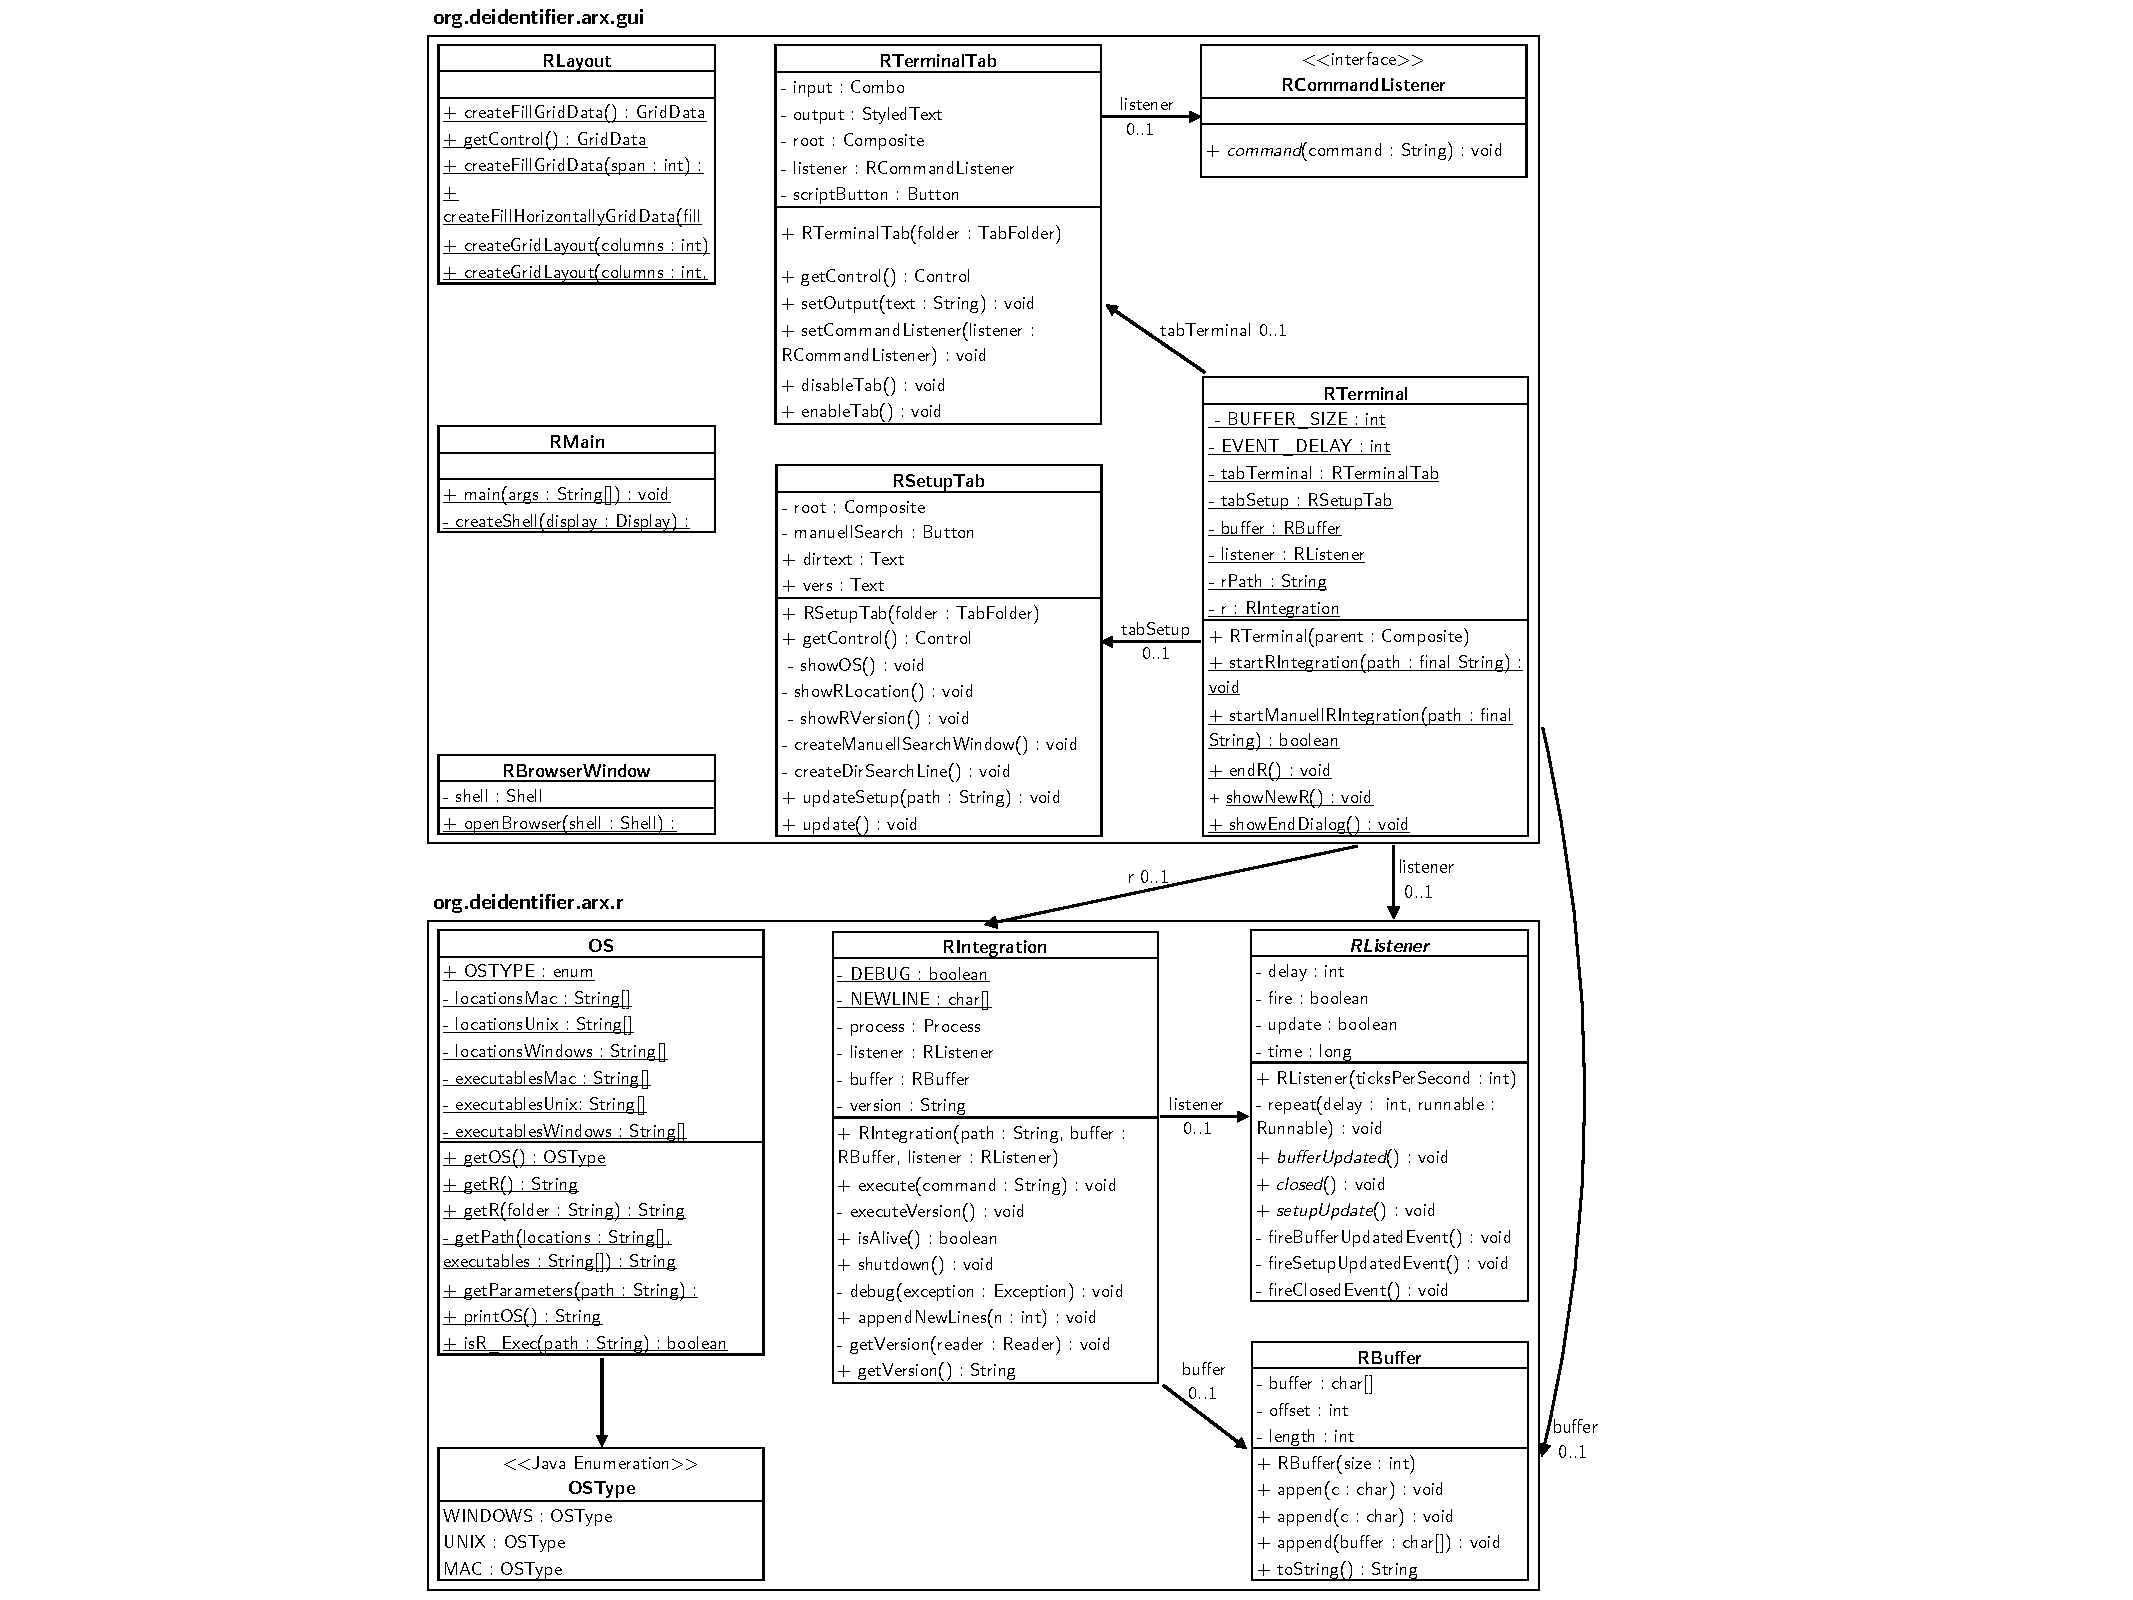
\includegraphics[width = 15cm]{Bilder/Klassendiagramm.pdf}
    	\caption{\textit{R-Terminal}: Klassendiagramm des Programms}
    	\label{klassendiagramm}
\end{figure}
\FloatBarrier
\newpage

\section{Graphische Benutzeroberfläche (GUI)}\label{gui}

\begin{samepage}

Das erste Package, "`org.deidentifier.arx.gui"', erzeugt und verwaltet die graphische Benutzeroberfläche. Es umfasst sieben Klassen:
\begin{itemize}
	\item RMain
	\item RTerminal
	\item RSetupTab
	\item RTerminalTab
	\item RBrowserWindow
	\item RLayout
	\item RCommandListener
\end{itemize}
\end{samepage}

\subsection{RMain}

Um das Programm mit einer graphischen Benutzeroberfläche zu starten, muss die "`main"'-Methode der Klasse \textit{RMain} ausgeführt werden. 

Diese erzeugt ein neues Display sowie eine Shell. Im Anschluss wird ein neues Objekt der Klasse \textit{RTerminal} erzeugt.

\subsection{RTerminal}

Die Erzeugung der einzelnen Komponenten der graphischen Benutzeroberfläche wird durch den Konstruktor der Klasse \textit{RTerminal} realisiert.\\

Dieser erzeugt einen TabFolder mit zwei Tabs, der erste Tab beinhaltet ein Objekt der Klasse \textit{RTerminalTab}, der zweite ein Objekt der Klasse \textit{RSetupTab}.
Außerdem erzeugt der Konstruktor noch einen Ring-Puffer der Klasse \textit{RBuffer} "`buffer"', welcher zur Speicherung des Std-Output von \textit{R} verwendet wird, sowie einen \textit{RListener} "`listener"'. Sowohl der Ring-Puffer, als auch der \textit{RListener} wurden im Package "`org.deidentifier.arx.r"' implementiert.
Im Konstruktor werden die abstrakten Methoden "`bufferUpdated()"', "`closed()"' und "`setupUpdate()"' überschrieben, sodass diese die Inhalte der beiden Tabs aktualisieren.\\

Im Anschluss wird die Integration mit \textit{R} durch den Aufruf der Methode "`startRIntergration"' eingeleitet.
Diese Methode "`startRIntergration"' erzeugt ein neues Objekt der Klasse "`RIntegration"', welches in \ref{RIntegration} beschrieben wird und die Integration von \textit{R} realisiert.


\subsection{RSetupTab}

Die Klasse \textit{RSetupTab} erzeugt einen Tab, welcher Informationen zum verwendeten Betriebssystem sowie dem aktuellen Status der Integration von \textit{R} anzeigt.\\

Die unterschiedlichen Informationen werden in \textit{SWT}-Labels dargestellt, welche in einem \textit{GridLayout} angeordnet sind.
Die \textit{SWT}-Labels werden durch die Methodenaufrufe "`showOS()"', "`showRLocation()"', "`showRVersion()"' im Konstruktor erzeugt.

Um das verwendete Betriebssystem abzufragen, wird die Methode "`printOS()"' der Klasse \textit{OS}, siehe \ref{OS}, von "`showOS()"' aufgerufen. Diese gibt das verwendete Betriebssystem als String zurück.

%Das aktuell verwendete Betriebssystem wird durch den Aufruf der Methode "`printOS()"' der Klasse \textit{OS} aus dem zweiten Package aufgerufen. Weitere Informationen hierzu finden sich in \ref{OS}.

Die Integration von \textit{R} wird in der Klasse \textit{RIntegration} des  Package "`org.deidentifier.arx.r"' umgesetzt. Diese wird beim Start des Programms in \textit{RTerminal} aufgerufen. 
 Um den Status der Integration zu prüfen, rufen "`showRLocation()"' und "`showRVersion()"' die Methode "`getR()"' aus \textit{OS} auf. Diese gibt den absoluten Pfad zur aktuell verwendeten R-Executive zurück, welcher im \textit{RSetupTab} angezeigt wird.
Wurde keine R-Executive gefunden oder konnte diese nicht erfolgreich gestartet werden, so wird von "`getR()"' \textit{null} zurückgegeben und im \textit{RSetupTab} wird ausgegeben:  
\begin{center}
Location: "`No valid R-exec found!"'

Version: "`No valid R-Version selected!"'
\end{center}
Wurde eine \textit{R}-Version gefunden und erfolgreich ausgeführt, so wird der erzeugte Listener in \textit{RTerminal} ausgelöst. Dieser ruft anschließend die Methode "`update()"' auf, durch welche der Inhalt von Location und Version aktualisiert wird.\\

Außerdem ermöglicht der \textit{RSetupTab} die manuelle Auswahl einer \textit{R}-Executive. Im Konstruktor wird hierfür ein Knopf mit "`createManuellSearchWindow()"' zum Öffnen eines Navigationsfensters sowie eine Kommandozeile "`createDirSearchLine()"' erzeugt, sodass entweder der absolute Pfad zur Datei angegeben oder diese mittels des Navigationsfensters ausgewählt werden kann.

Die Kommandoleiste wird in der Methode "`createDirSearchLine()"' erzeugt und erfasst die Eingabe durch einen \textit{TraverseListener}. Der \textit{TraverseListener} wird durch Drücken der Return-Taste ausgelöst und gibt den eingegeben Pfad an die Methode "`updateSetup($String$ path)"' weiter. Wird die \textit{R}-Executive mit dem Navigationsfenster gesucht, so wird der absolute Pfad der ausgewählten Datei ebenfalls an "`updateSetup($String$ path)"' als Argument übergeben. Nähere Informationen zum Navigationsfenster finden sich in \ref{RBrowserWindow}.

Die Methode "`updateSetup($String$ path)"' startet eine neue Integration von \textit{R} durch den Aufruf der Methode "`startManuellRIntegration($String$ path)"' aus der Klasse \textit{RTerminal}. Nähere Details hierzu in \ref{RTerminal}. 

Falls die \textit{R}-Executive erfolgreich gestartet wurde, wird durch den \textit{RListener} (siehe oben) der Tab wieder aktualisiert. Andernfalls wird die selbe Ausgabe angezeigt, wie bei der automatischen Suche.

\subsection{RTerminalTab} \label{RTerminal}

Im \textit{RTerminalTab} werden \textit{R}-Befehls-Eingaben des Nutzers erfasst sowie der Std-Output von \textit{R} ausgegeben. Außerdem können mittels eines Knopfes fertige \textit{R}-Skripte geladen und ausgeführt werden. Der \textit{RTerminalTab} ist nur nutzbar, falls \textit{R} erfolgreich gestartet und integriert wurde.\\

Der Tab hat als Layout ebenso wie der \textit{RSetupTab} ein \textit{GridLayout}.
Dieses besteht aus einem \textit{Composite} und einem Textfeld.\\

Das Kompositum "`topline"' umfasst eine Kommandozeile, ein Dropdown-Menü um eingegebene Befehle erneut auszuführen sowie einen Knopf zum Aufrufen von \textit{R}-Skripten. Als Layout wurde ebenfalls \textit{GridLayout} gewählt, da es alle Komponenten möglichst kompakt darstellt.

Die Kommandozeile und das Dropdown-Menü "`input"' wurden mit der importierten Klasse \textit{swt.widget.Combo} erstellt. Die Kommandozeile erfasst die Eingaben des Nutzers beim Drücken der Enter-Taste durch einen \textit{TraverseListener}. Die Eingabe wird anschließend an die Methode "`command($String$ command)"' der Klasse  \textit{RCommandListener} übergeben, welche den Befehl an \textit{R} übergibt. Dies wird in \ref{RCommandListener} genauer beschrieben.

Die letzten 10 eingegebenen Befehle werden im Dropdown-Menü angezeigt. Die Befehle werden in einem Ring-Puffer mit 10 Elementen gespeichert, welcher als String Array implementiert wurde.\\

Skripte können durch den Knopf "`scriptButton"' ausgewählt und ausgeführt werden. Der Knopf wird durch einen \textit{MouseListener} ausgelöst und erzeugt ein Navigationsfensters der Klasse \textit{RBrowserWindow}. Weiter Informationen hierzu in \ref{RBrowserWindow}. Durch dieses kann das Skript ausgewählt werden und es wird vom \textit{RBrowserWindow} der absolute Pfad des Skriptes übergeben. Anschließend wird überprüft, ob es sich um ein \textit{R}-Skript handelt, also die Datei auf "`.r"' endet. Trifft dies zu, so wird durch die Methode "`command($String$ command)"' der Klasse  \textit{RCommandListener} der Befehl das Skript zu öffnen an \textit{R} übergeben. Dieser setzt sich zusammen aus:
\begin{center}
$source("$  absoluter Pfad $")$
\end{center}

Das Textfeld "`output"' beinhaltet die Ausgabe von \textit{R} und wurde durch die importierte Klasse \textit{StyledText} realisiert. Das Textfeld ist als Ring-Puffer implementiert, sodass dieser nur die letzten $10000$ Zeichen des \textit{R}-Std-Output anzeigt. Die Größe des Ring-Puffers ist in der Klasse \textit{RTerminal} als globale int Variable "`BUFFER\_SIZE"' festgelegt und kann hier geändert werden.
Der Std-Output von \textit{R} wird durch das Auslösen des RListener "`listener"' in \textit{RTerminal} aktualisiert. Dieser ruft hierzu die Methode "`setOutput($String$ text)"' aus \textit{RTerminalTab} auf. Der Listener wird nach erfolgreichem Starten von \textit{R} durch die Klasse \textit{RIntegration} übergeben. Diese ruft die Methode "`setCommandListener($RCommandListener$ listener)"' im \textit{RTerminalTab} auf und übergibt den Listener als Argument. Details zum Listener finden sich in \ref{RCommandListener}.\\

Außerdem wird nach einem erfolgreich Start von \textit{R} durch "`startRIntegration($String$ path)"' aus der Klasse \textit{RTerminal}  die Methode "`enableTab()"' in \textit{RTerminalTab} aufgerufen, sodass der Tab nutzbar wird. Beim Beenden von \textit{R} wird in der Methode "`endR()"' in  \textit{RTerminal} die Methode "`disableTab()"' in \textit{RTerminalTab} aufgerufen, welche den Tab wieder für den Nutzer sperrt.

\subsection{RBrowserWindow} \label{RBrowserWindow} 

Die Klasse \textit{RBrowserWindow} implementiert ein Navigationsfenster des Standart-Dateimanagers. 
Dieses wurde durch die importierte \textit{SWT}-Klasse \textit{FileDialog} implementiert. Die Klasse beinhaltet nur eine Methode "`openBrowser(Shell)"', durch welche ein neuer \textit{FileDialog}, also ein Navigationsfenster, erzeugt wird, mit welchem eine Datei ausgewählt werden kann. Anschließend gibt die Methode den absoluten Pfad der ausgewählten Datei zurück. 
Mit dem Navigationsfenster kann sowohl manuell die \textit{R}-Executive im \textit{RSetupTab} sowie ein ausführbares \textit{R}-Skript im \textit{RTerminalTab} ausgewählt werden. Anschließend wird der absolute Pfad per \textit{return} übergeben, sodass der funktionale Kern, siehe \ref{funktionaler Kern}, die jeweilige Aktion durchführen kann.

\subsection{RLayout}

Diese Klasse definiert das \textit{SWT}-Layout der Klassen \textit{RSetupTab} und \textit{RTerminalTab}. 
Die Methoden der Klasse werden im Konstruktur der beiden genannten Klassen aufgerufen, um die \textit{SWT}-Objekte der des jeweiligen Tabs mit den richtigen Parametern und Abständen zu erzeugen.

\subsection{RCommandListener} \label{RCommandListener}

Das \textit{Java}-Interface \textit{RCommandListener} implementiert einen Listener, welcher bei der Eingabe von Befehlen für \textit{R} ausgeführt wird. Die abstrakte Methode "`command($String$ command)"' des Interfaces wird in der Klasse \textit{RTerminal} mit der Methode "`execute(command)"' aus der Klasse \textit{RIntegration} überschrieben. Somit wird die Trennung der graphischen Oberfläche und des funktionalen Kerns der \textit{R}-Integration, welcher in \ref{funktionaler Kern} beschrieben wird, beibehalten.


\section{Funktionaler Kern - Integration von R} \label{funktionaler Kern}

Die Integration von \textit{R} in \textit{Java} ist in dem Package "`org.deidentifier.arx.r"' implementiert. Dieses beinhaltet alle Funktionen, durch welche die \textit{R}-Executive automatisch gefunden, ausgeführt und das Betriebssystem erkannt wird. Außerdem beinhaltet es alle Methoden zur Übermittlung des Input- und Outputstreams.
Zur Integration von \textit{R} in \textit{Java} wurde die Klasse \textit{ProcessBuilder} \cite{processBuilder} verwendet.

\begin{samepage}
Das Package umfasst vier Klassen:
\begin{itemize}
	\item RIntegration
	\item OS
	\item RBuffer
	\item RListener
\end{itemize}
\end{samepage}


\subsection{RIntegration} \label{RIntegration}

Die Klasse \textit{RIntegration} ist das Kernstück des \textit{R-Terminals} und ist für die Integration von \textit{R} verantwortlich. Der \textit{R}-Prozess wird durch die Library \textit{ProcessBuilder} \cite{processBuilder} gestartet.

Wird das Programm mit der graphischen Benutzeroberfläche gestartet, so wird für jede gefundene ausführbare \textit{R}-Executive durch die Methode "`startRIntegration"' beziehungsweise "`startManuellRIntegration"' ein neues Objekt dieser Klasse erzeugt.
Hierbei werden dem Konstruktor folgende Argumente übergeben:
\begin{itemize}
	\item $final$ $String$ path
	\item $final$ $buffer$ buffer 
	\item $final$ $RListener$ listener
\end{itemize}
%
Der absolute Pfad zur Executive wird durch "`path"' angegeben. Bei "`buffer"' handelt es sich um den Ring-Puffer der Klasse \textit{RBuffer}, welcher zur Ausgabe des Std-Output des \textit{R}-Prozesses im \textit{RTerminalTab} erzeugt wurde. Gibt es eine neue Ausgabe des Std-Output des Prozesses, so wird dieser im Ring-Puffer angehängt. 
Um die beiden Tabs \textit{RSetupTab} und \textit{RTerminalTab} bei Änderungen zu aktualisieren, wird der \textit{RListener}, welcher in \textit{RTerminal} erzeugt wurde, als Attribut "`listener"' übergeben.
Bei einer Ausgabe des Std-Output oder Start bzw. Beenden des \textit{R}-Prozesses wird dieser ausgelöst.\\

Der Konstruktor erzeugt ein neues Objekt der Klasse \textit{ProzessBuilder} mit den betriebssystemspezifischen Parametern. Die Parameter werden durch Aufrufen der Methode "`getParameters($String$ path)"', siehe \ref{OS}, aus der Klasse \textit{OS} übergeben und dem Konstruktor des \textit{ProzessBuilders} als Argumente übergeben.

Anschließend wird der Prozess gestartet.\\

Nach erfolgreichen Start des \textit{R}-Prozesses wird ein Reader "`reader"' erzeugt, welchem die Ausgabe des \textit{R}-Prozesses übergeben wird. Dieser Reader übergibt die Ausgabe an den Ring-Puffer "`listener"'.

Direkt im Anschluss wird die Methode "`getVersion($Reader$ reader)"' aufgerufen. Durch diese wird abgefragt, welche Version von \textit{R} verwendet wird.
Die Ausgabe der Version wird durch das Kommando "`version"', welches an den laufenden \textit{R}-Prozess als Input durch den Methodenaufruf "`execute("version")"' übergeben wird, erreicht. Die Ausgabe dieses Kommandos soll nicht im Ausgabefenster der GUI, dem \textit{RTerminalTab}, angezeigt werden. Deshalb erzeugt die Methode "`getVersion(Reader reader)"' einen neuen, temporären Ring-Puffer, in welchem die Ausgabe für diesen Befehl gespeichert wird. 

Aus dem Ausgabe-String dieses "`version"'-Kommandos wird anschließend die genaue Version sowie der Nickname extrahiert und in der lokalen Variable "`version"' gespeichert. Im Anschluss wird der Rlistener  "`listener"' ausgelöst, welcher die Methode "`setupUpdate()"' ausführt. Diese Methode ruft die "`update"'-Methode im \textit{RSetupTab} auf und aktualisiert den Tab.\\

Nach Abschluss dieses Kommandos wird die gesamte Ausgabe in den Ring-Puffer "`buffer"' geschrieben und durch Auslösen des RListener "`listener"' in dem Ausgabefenster des \textit{RTerminalTabs} angezeigt.\\

Kommandos, welche in \textit{R} ausgeführt werden sollen, werden als String der Methode "`execute($String$ command) "' übergeben, welche diese an den \textit{R}-Prozess weiterleitet. Hier wird ein \textit{BufferedWriter}-Objekt erstellt. Mit der "`write(String command)"' Methode dieses Elementes wird das Kommando in dem \textit{BufferedWriter} geschrieben und anschließend mit "`newline()"' noch ein Zeilenumbruch im \textit{BufferedWriter} gespeichert. Um den Inhalt des \textit{BufferedWriter} an den \textit{R}-Prozess zu übergeben, diesen auszuführen und anschließend den \textit{BufferedWriter} zu leeren, wird zum Abschluss die Methode "`flush()"' aufgerufen.
Mit dieser Methode werden alle Kommandos an den \textit{R}-Prozess übergeben. Die "`execute($String$ command)"' Methode wird bei der Nutzung der GUI von der Methode "`command($String$ command)"' aufgerufen. Nähere Informationen zur Methode "`command($String$ command)"' finden sich in \ref{RCommandListener}.

\subsection{OS} \label{OS}

Die Klasse \textit{OS} implementiert folgende Funktionalitäten: Erkennung des verwendeten Betriebsystems, die Anpassung der Pfade der Standard-Speicherorte der \textit{R}-Executive je nach verwendeten Betriebssystem und die Überprüfung der übergebenen \textit{R}-Executives.\\

Um die drei unterstützten Betriebssysteme Windows, Mac und Unix effizient zu unterscheiden, werden diese als Enum Konstanten "`OSType"' erzeugt.\\

Die absoluten Pfade der Standart-Speicherorte der \textit{R}-Executive werden für jedes Betriebssystem in einem eigenen String Array gespeichert. Es ist wichtig hier zu beachten, dass Windows andere Separatoren verwendet als Linux und OS X.
Bei Windows müssen die einzelnen Verzeichnisse durch "`$\backslash \backslash$"' getrennt werden, bei beiden anderen Betriebssystemen durch "`/"'. 

Falls neue Standart-Speicherorte für die \textit{R}-Executive hinzugefügt werden sollen, kann das jeweilige Array einfach um den neuen Pfad erweitert werden. Beim Starten des \textit{R-Terminals} durch die graphische Benutzeroberfläche werden alle Pfade des Arrays nach einer ausführbaren \textit{R}-Executive durchsucht. Hierfür wird die Methode "`getR()"' aufgerufen, welche im Folgenden noch vorgestellt wird.\\

Außerdem werden die Dateinamen der \textit{R}-Executive für die unterschiedlichen Betriebssysteme in einem String-Array gespeichert, da sich diese je nach Betriebssystem unterscheiden. Außerdem wird das jeweilige Array benötigt, um bei der manuellen \textit{R}-Auswahl zu prüfen, ob es sich um eine gültige \textit{R}-Executive handelt. Dies wird in der Methode "`isRExec($String$ path)"' in Abhängigkeit vom verwendeten Betriebssystems überprüft.\\

Die Methode "`getOS()"' fragt den Namen des Betriebssystems ab und gibt dieses als Enum "`OSType"' passend zurück.\\

Wie bereits beschrieben, werden nach dem Start des Programms die Standart-Speicherorte nach einer ausführbaren R-Executive durchsucht. Ob an einem dieser Speicherorte eine Executive liegt, wird mit der Methode "`getPath($String[]$ locations, $String[]$ executables)"' überprüft. Außerdem wird versucht die Executive mit \textit{ProcessBuilder} zu starten, um zu prüfen, ob der Nutzer ausreichende Zugriffsberechtigungen besitzt.\\

Zusätzlich sind in der Klasse \textit{OS} die Parameter zur Ausführung der \textit{R}-Executive für den \textit{ProcessBuilder} gespeichert. Diese werden beim Aufruf der Methode "`getParameters($String$ path)"' mit dem Pfad "`path"' der Executive zu einem String-Array konkateniert und anschließend als String Array zurückgegeben.

\subsection{RBuffer} \label{RBuffer}

Diese Klasse implementiert den Ring-Puffer, welcher für die Ausgabe des Std-Output von \textit{R} im Ausgabefenster des \textit{RTerminalTab} verwendet wird.
Die Größe des Ring-Puffers wird bei der Erzeugung dem Konstruktor übergeben und ist beim Starten des Programms mit graphischer Benutzeroberfläche in der Klasse \textit{RTerminal} in der Variable "`BUFFER\_SIZE"' festgelegt.

\subsection{RListener} \label{RListener}

Die Klasse \textit{RListener} implementiert einen Listener, welcher in den Klassen \textit{RTerminal}, siehe \ref{gui}, sowie \textit{RIntegration} verwendet wird. \\

Der Listener aktualisiert die Inhalte von \textit{RSetupTab} sowie \textit{RTerminalTab}. 
Durch die abstrakte Methode "`setupUpdate()"', welche in \textit{RTerminal} überschrieben wird, wird bei Änderung des Status von \textit{R}, also dem Beenden oder dem Starten eines neuen \textit{R}-Prozesses der \textit{RSetupTab} aktualisiert.
Durch "`bufferUpdate()"' wird das Ausgabefenster im \textit{RTerminalTab} aktualisiert. Diese abstrakte Methode wird ebenfalls in \textit{RTerminal} überschrieben.



\section{Ausführung ohne graphische Benutzeroberfläche} \label{ohne GUI}

Der funktionale Kern des \textit{R-Terminals} kann auch ohne die graphische Benutzeroberfläche ausgeführt werden. 
Hierfür wird die Umsetzung anhand eines Beispiels in \ref{BeispielOhneGUI} erklärt. 
Eine Übersicht der Methoden zur Nutzung des \textit{R-Terminals} ohne GUI befindet sich in \ref{API}.

\subsection{Aufruf des R-Terminals ohne GUI} \label{BeispielOhneGUI}

Um das \textit{R-Terminal} ohne graphische Benutzeroberfläche zu nutzen müssen folgende Objekte erzeugt werden:
\begin{itemize}
	\item ein Ring-Puffer der Klasse \textit{RBuffer}, welcher der Std-Output von \textit{R} übergeben wird
	\item ein Listener der Klasse \textit{RListener}, welcher durch den Std-Output ausgelöst wird
\end{itemize}
	
Anschließend müssen die abstrakten Methoden des \textit{RListeners} überschrieben werden:
	\begin{itemize}
		\item \textit{bufferUpdated()}
		\item \textit{closed()}
		\item \textit{setupUpdate()}
	\end{itemize}

Nun kann die Integration von \textit{R} gestartet werden. Hierfür muss ein neues \textit{RIntegration}-Objekt erzeugt werden. Diesem werden der Pfad "`path"' zur \textit{R}-Executive als String, der erzeugte \textit{RBuffer} "`buffer"' und der \textit{RListener} "`listener"' übergeben:

\lstset{language=Java}
\begin{lstlisting}[frame=single]
final RIntegration rProcess = 
	new RIntegration(path, buffer, listener)	
\end{lstlisting}

Um dem \textit{R}-Prozess nun Befehle zu übergeben, muss lediglich die Methode "`execute"' des erzeugten \textit{RIntegration}-Objekt aufgerufen werden und das Kommando als String übergeben werden.\\
\\
Beispiel: Es wurde ein \textit{RIntegration}-Objekt \textit{rProcess} erzeugt und es soll "`1+2+3+4+5"' als Kommando übergeben werden, dann muss

\lstset{language=Java}
\begin{lstlisting}[frame=single]
rProcess.execute("1+2+3+4+5")	
\end{lstlisting}
ausgeführt werden. Die Ausgabe wird im Ring-Puffer gespeichert, welcher für den Std-Output erzeugt wurde.\\
\\
Ein Code-Beispiel hierzu befindet sich im Package "`ExampleWithoutGUI"'.

\subsection{API} \label{API}

\subsection{Klasse: RIntegration}

\lstset{language=Java}
\begin{lstlisting}[frame=single]
public RIntegration(final String path, 
	            final RBuffer buffer,
	            final RListener listener)	
\end{lstlisting}
%
Der Konstruktor dieser Klasse erzeugt den \textit{R}-Prozess, startet diesen und verwaltet die Input- und Outputstreams.
\begin{itemize}
	\item path: String des Pfades zur \textit{R}-Executive
	\item buffer: Output-Buffer
	\item listener: Listener des Std-Outputstreams des \textit{R}-Prozess
\end{itemize}

\lstset{language=Java}
\begin{lstlisting}[frame=single]
public void execute(String command)
\end{lstlisting}
\begin{itemize}
	\item command: Das Kommando als String
\end{itemize}

Durch die Methode "`execute"' werden die Befehle für den \textit{R}-Prozess ausgeführt.
%
\lstset{language=Java}
\begin{lstlisting}[frame=single]
public boolean isAlive()
\end{lstlisting}
%
Mit der Methode "`isAlive"'  kann geprüft werden, ob der \textit{R}-Prozess noch aktiv ist.
\begin{itemize}
	\item returns true: \textit{R}-Prozess ist noch aktiv
	\item returns false: \textit{R}-Prozess ist nicht mehr 
\end{itemize}


\lstset{language=Java}
\begin{lstlisting}[frame=single]
public void shutdown()
\end{lstlisting}
%
Die Methode "`shutdown"' beendet den laufenden \textit{R}-Prozess.\\

\lstset{language=Java}
\begin{lstlisting}[frame=single]
public String getVersion()
\end{lstlisting}
%
Die Methode "`shutdown"' gibt die Version und den Nickname der letzten verwendeten \textit{R}-Version konkateniert als String zurück.

\subsection{Klasse: OS}

\lstset{language=Java}
\begin{lstlisting}[frame=single]
public static OSType getOS()
\end{lstlisting}
Diese Methode gibt das verwendete Betriebssystem zurück:
\begin{itemize}
	\item Enum OSType (WINDOWS,UNIX,MAC)
\end{itemize} 
Wird das Betriebssystem nicht unterstützt, wird folgende Exception geworfen:
\begin{itemize}
	\item IllegalStateException("{}Unsupported operating system"{})
\end{itemize}

 
\lstset{language=Java}
\begin{lstlisting}[frame=single]
public static String getR()
\end{lstlisting}
\begin{itemize}
	\item returns \textit{String} path: gibt den Pfad zur gefundenen \textit{R}-Executive als String zurück
	\item returns \textit{null}: falls keine Executive gefunden wurde
\end{itemize}


\lstset{language=Java}
\begin{lstlisting}[frame=single]
public static String getR(String folder)
\end{lstlisting}
Diese Methode durchsucht das übergebene Verzeichnis nach einer \textit{R}-Executive
\begin{itemize}
	\item returns \textit{String} path: Falls eine Executive gefunden wurde wird der absolute Pfad zu dieser zurückgegeben
	\item returns \textit{null}: Falls keine Executive gefunden wurde
\end{itemize}


\lstset{language=Java}
\begin{lstlisting}[frame=single]
public static String[] getParameters(String path)
\end{lstlisting}
Die Methode "`getParameters"' gibt die Parameter für den \textit{ProcessBuilder} aus.
\begin{itemize}
	\item path: Der Pfad zur \textit{R}-Executive 
	\item MAC: returns $String$[] \{path, "--vanilla", "--quiet", "--interactive" \};
	\item UNIX: returns $String$[] \{path, "--vanilla", "--quiet", "--interactive" \};
	\item WINDOWS: returns $String$[] \{path, "--vanilla", "--quiet", "--ess"\};
\end{itemize}

\lstset{language=Java}
\begin{lstlisting}[frame=single]
public static String printOS()
\end{lstlisting}
Diese Methode gibt das verwendete Betriebssystem als String zurück.
\begin{itemize}
	\item returns: "macOS", "{}Unix", "Windows"
	\item IllegalStateException("{}Unknown operating system"): falls das OS nicht zu den drei oben genannten gehört
\end{itemize}

\lstset{language=Java}
\begin{lstlisting}[frame=single]
public static boolean isR_Exec(String path)
\end{lstlisting}
Diese Methode prüft, ob die übergebene Datei eine \textit{R}-Executive ist.
\begin{itemize}
	\item $String$ path: der absolute Pfad der Datei
	\item returns $true$: Datei ist eine \textit{R}-Executive
	\item returns $false$: Datei ist keine \textit{R}-Executive
\end{itemize}

\subsection{Klasse: RBuffer}

\lstset{language=Java}
\begin{lstlisting}[frame=single]
public RBuffer(int size)
\end{lstlisting}
Dem Konstruktor wird die Größe des Ring-Puffers als Anzahl der Zeichen übergeben.\\

\lstset{language=Java}
\begin{lstlisting}[frame=single]
public void append(char c)
\end{lstlisting}
Fügt ein Zeichen an den Ring-Puffer an.\\

\lstset{language=Java}
\begin{lstlisting}[frame=single]
public void append(char[] buffer)
\end{lstlisting}
Fügt alle im Char-Array enthaltenen Zeichen an den Ring-Puffer an.\\

\lstset{language=Java}
\begin{lstlisting}[frame=single]
public String toString()
\end{lstlisting}
Diese Methode gibt den gesamten Inhalt des Ring-Puffers als String zurück.

\subsection{Klasse: RListener}

\lstset{language=Java}
\begin{lstlisting}[frame=single]
public RListener(int ticksPerSecond)
\end{lstlisting}
Dem Konstruktor wird die maximale Anzahl an Events pro Sekunde als int übergeben.\\
\\
Die folgenden drei abstrakten Methoden müssen beim erzeugen eines neuen \textit{RListener}-Objetes überschrieben werden.

\lstset{language=Java}
\begin{lstlisting}[frame=single]
public abstract void bufferUpdated();
\end{lstlisting}
Diese Methode wird bei einem Update des Output-Buffers ausgelöst.\\

\lstset{language=Java}
\begin{lstlisting}[frame=single]
public abstract void closed();
\end{lstlisting}
Diese Methode wird beim Beenden des \textit{R}-Prozesses ausgelöst.\\

\lstset{language=Java}
\begin{lstlisting}[frame=single]
public abstract void setupUpdate();
\end{lstlisting}
Diese Methode wird beim Starten eines neuen \textit{R}-Prozesses ausgelöst.


\section{Abhängigkeiten} \label{Abhängigkeiten}

Das Projekt beinhaltet bereits alle benötigten \textit{Java}-Libraries zur Ausführung der Software. 
Da die graphische Benutzeroberfläche mit \textit{SWT} realisiert wurde, müssen die \textit{SWT}-Libraries je nach Betriebssystem ausgewählt werden. Dies wird genauer unter \ref{swt} erläutert.\\

Für die Integration von \textit{R} in \textit{Java}, welche durch das \textit{R-Terminal} umgesetzt wurde, muss eine Standalone-Installation von \textit{R} vorliegen. 
 
\subsection{Java}

Die für das \textit{R-Terminal} verwendetet Programmiersprache ist \textit{Java}. Für die Entwicklung und Tests wurde \textit{Java SE 8 (1.8.0\_91)} verwendet. \cite{java}
 
\subsection{R-Project} \label{r}

Um \textit{R} in \textit{Java} zu integrieren muss eine Standalone-Installation von R, für welche der aktuellen Benutzer ausreichende Zugriffsrechte besitzt, vorhanden sein. 
Alle aktuellen \textit{R}-Versionen können von der Homepage des \textit{R}-Projects \cite{rproject} heruntergeladen werden. 


\subsection{SWT}\label{swt} 
Die graphische Benutzeroberfläche wurde mithilfe des \textit{Standard Widget Toolkit} (\textit{SWT}) realisiert \cite{swt}. \textit{SWT} ist ein "`open-source widget toolkit"' für Java mit Integration in die GUI des nativen Betriebssystems, sodass das Design der Benutzeroberfläche an das Design des Betriebssystems angepasst wird. 

Für das Projekt \textit{R-Terminal} wurde die \textit{SWT}-Version 4.2.1 verwendet.\\

Wie die betriebssystemspezifischen \textit{SWT}-Libraries auf den "`Build Path"' hinzugefügt werden, kann unter \ref{swtanwender} nachgeschlagen werden.

%---------------------Ergebnis----------------------------


\chapter{Ergebnis}
\section{Übersicht}
Das \textit{R-Terminal} dient dazu, über eine externe Schnittstelle \textit{R} aufzurufen und zu bedienen. Dies soll vor allem dazu genutzt werden, um Tabellen aus \textit{ARX} einzuladen, auf diesen Skripte auszuführen, und gleichzeitig die in der Einleitung beschriebenen Probleme zu umgehen. Das \textit{R-Terminal} ist kompatibel mit Windows, der Linux Distribution Ubuntu und OS X, von denen jeweils die folgenden Versionen im Rahmen der Entwicklung getestet wurden: 

\begin{itemize}
\item Windows 10 Education (Version 1511)
\item OS X El Capitan (Version 10.11.1)
\item macOS Sierra (Version 10.12.2)
\item Ubuntu
\end{itemize}

%insert screenshot for linux and the correct ubuntu/opensuse version

In den folgenden Abschnitten werden die Grundfunktionen und zusätzliche Features des \textit{R-Terminals} beschrieben. 

\section{Voraussetzungen}

Um die Software \textit{R-Terminal} auszuführen, muss \textit{Java} sowie eine Standalone-Installation von \textit{R} installiert sein. Es wird empfohlen das \textit{R-Terminal} mit Eclipse auszuführen.
Die Versionen, mit welchen die Software getestet wurde, sind unter \ref{Abhängigkeiten} aufgeführt. 

\section{Vorbereitung} \label{swtanwender}

Zunächst muss  das Projekt \textit{R-Terminal} in Eclipse importiert werden.

Um das \textit{R-Terminal} ausführen zu können, müssen die betriebssystemspezifischen \textit{SWT}-Libraries auf den Build-Path gesetzt und die \textit{SWT}-Libraries anderer Betriebssysteme entfernt werden.
Im Folgenden wird genau beschrieben, wie dies unter \textit{Eclipse} umgesetzt wird:
\begin{enumerate}
	\item Navigieren Sie im \textit{Eclipse} Package Explorer zu:
	\begin{center}\textit{R-Terminal -> lib  -> swt} \end{center}
	
	\item Wählen Sie die betriebssystemspezifischen \textit{SWT}-Libraries aus und öffnen Sie mit der rechten Maustaste, bzw. dem OS-spezifischen Äquivalent, für jede dieser Libraries das Auswahlfenster. Klicken Sie auf "`Build-Path"'.
		Sollte die Library bereits hinzugefügt sein, erscheint "`Configure Build Path..."'. Ist dies nicht der Fall, erscheint "`Add to Build Path"', klicken Sie dieses an. Die beiden Fälle werden  in Abbildung \ref{addToBuildPath} und \ref{onBuildPath} dargestellt.  \\

\begin{figure}
\centering	
	\begin{minipage}{0.5\textwidth}
	\centering	
		\captionsetup{width=0.9\linewidth}
		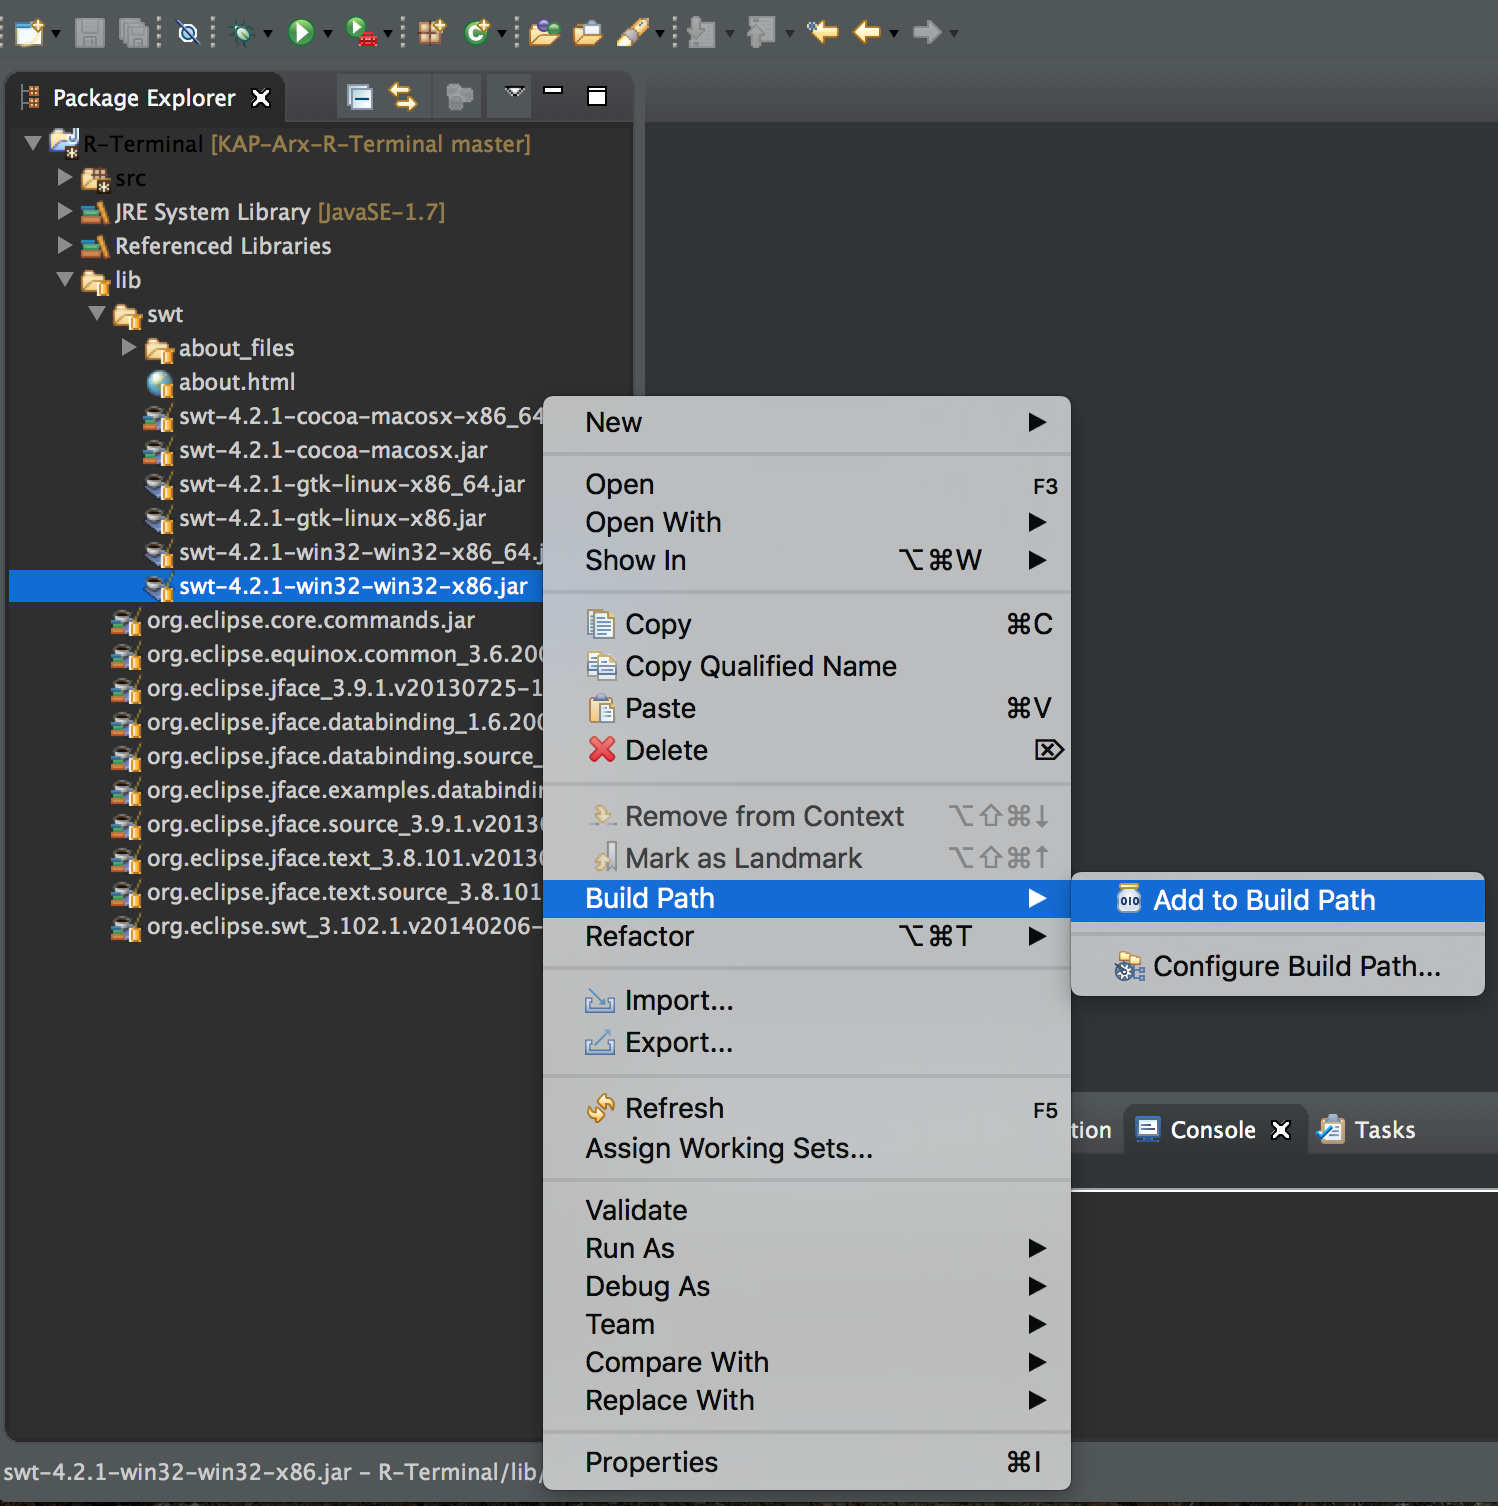
\includegraphics[width=0.9\linewidth]{Bilder/SWT-Add-to-Build-Path}
    	\caption{\textit{Eclipse}: Hinzufügen der \textit{SWT}-Library zum Build Path}
    	\label{addToBuildPath}
	\end{minipage}%
	\begin{minipage}{0.5\textwidth}
	\centering
		\captionsetup{width=0.9\linewidth}
    	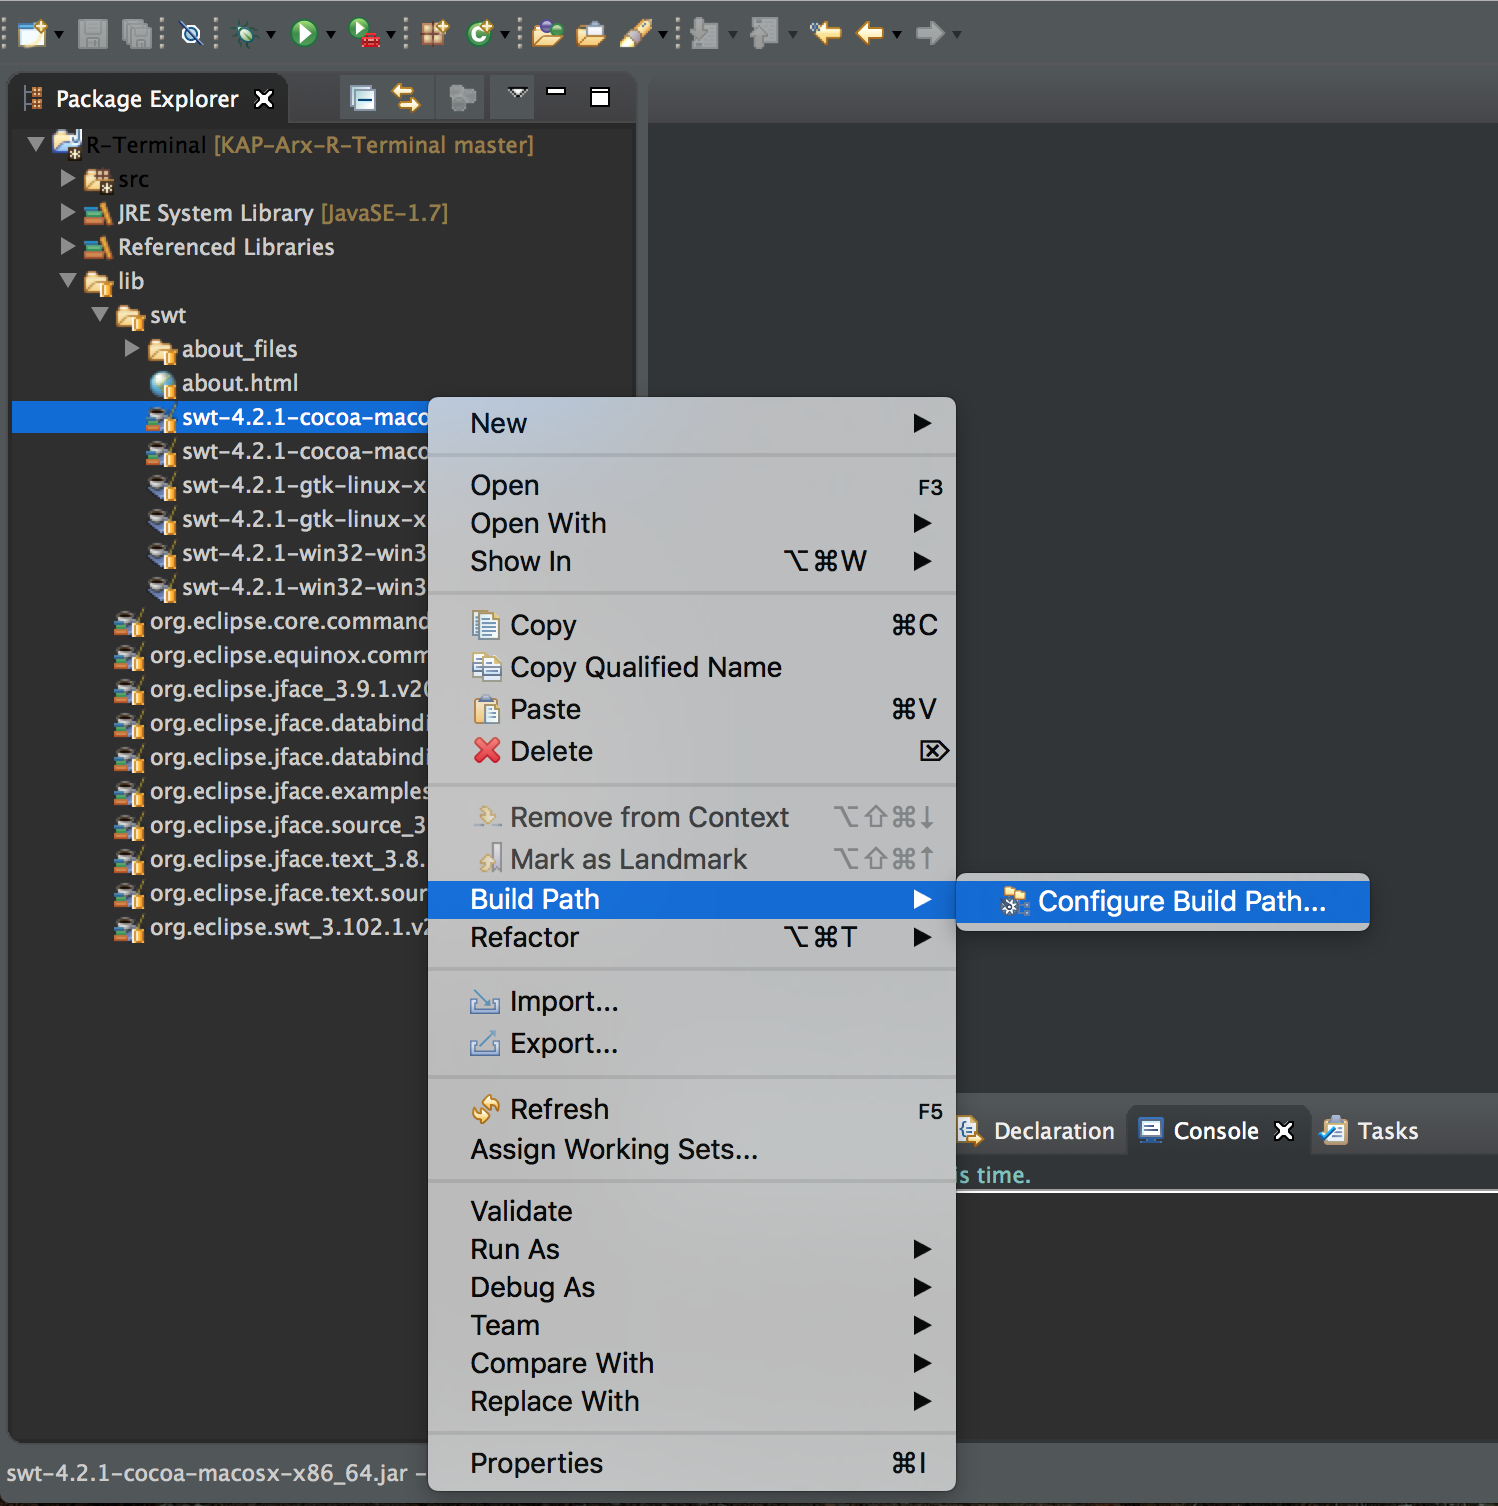
\includegraphics[width=0.9\linewidth]{Bilder/SWT-Configure-Build-Path}
    	\caption{\textit{Eclipse}: Diese \textit{SWT}-Library ist bereits auf dem Build Path}
    	\label{onBuildPath}
	\end{minipage}
\end{figure}
		
	Betriebssystemspezifische \textit{SWT}-Libraries:
		
	\begin{itemize}
		\item Windows: \begin{itemize}
							\item swt-4.2.1-win32-win32-x86\_64.jar
							\item swt-4.2.1-win32-win32-x86.jar
						\end{itemize}
						
		\item Mac: \begin{itemize}
						\item swt-4.2.1-cocoa-macosx-x86\_64.jar
						\item swt-4.2.1-cocoa-macosx.jar
					\end{itemize}
		\item Linux: \begin{itemize}
						\item swt-4.2.1-gtk-linux-x86\_64.jar
						\item swt-4.2.1-gtk-linux-x86.jar
					 \end{itemize}
	\end{itemize} 
	
	\item Überprüfen Sie nun, ob alle anderen Libraries des Ordners \textit{swt} nicht auf dem "`Build Path"' liegen. 
		Gehen Sie hierfür zu:
		\begin{center}
			\textit{R-Terminal -> Referenced Libraries}
		\end{center} 
		
		Überprüfen Sie, dass keine der genannten Libraries der oberen Aufzählung, die nicht Ihrem Betriebssystem zugehört, in diesem Ordner enthalten ist.
		Sollte sich eine \textit{SWT}-Library für ein anderes Betriebssystems in diesem Ordner befinden, öffnen Sie mit einem Rechtsklick das Menü und wählen Sie aus: 
		\begin{center}
			\textit{Build Path -> Remove from Build Path}
		\end{center}	
		Dies wird auch in Abbildung \ref{removeFromBuildPath} dargestellt.
		
		Nun können Sie das \textit{Java}-Programm Sie die "`main"'-Methode in \textit{RMain} ausführen.
\end{enumerate}
\begin{figure}[t]
	\centering
		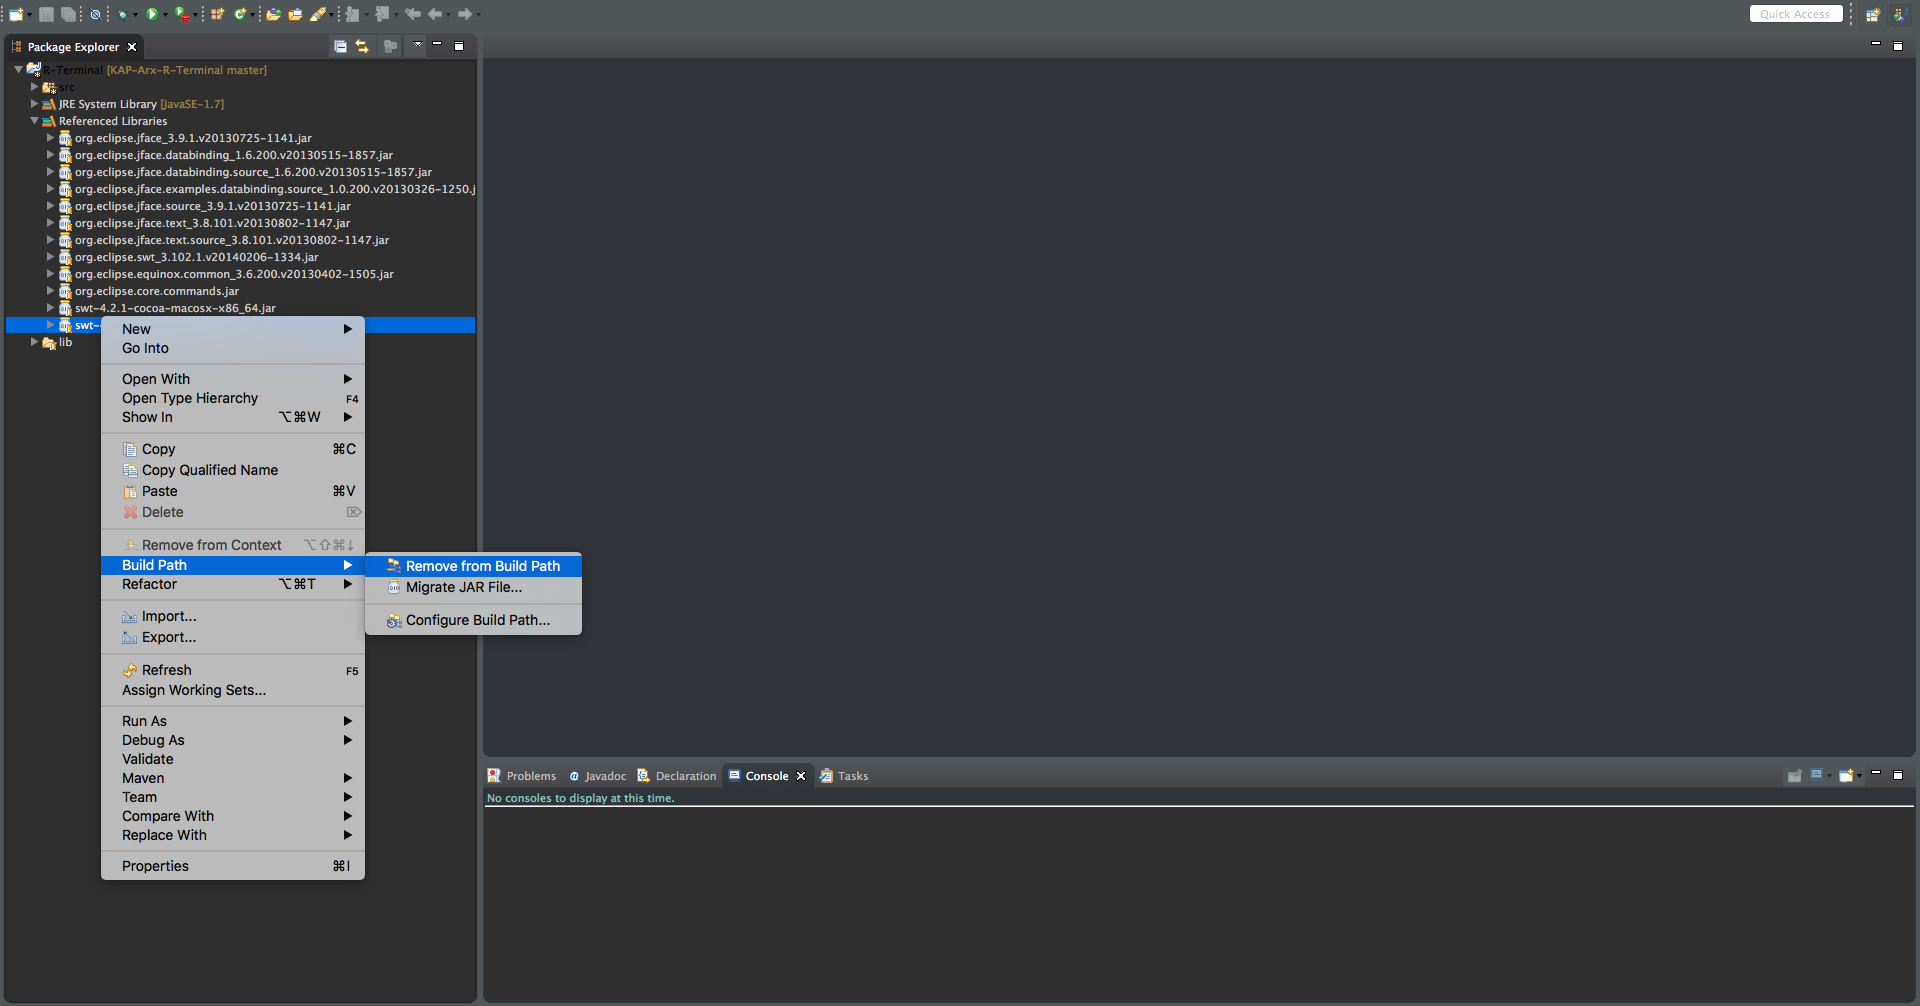
\includegraphics[width=\linewidth]{Bilder/SWT-Remove-from-Build-Path}
    	\caption{\textit{Eclipse}: Entfernen der \textit{SWT}-Library vom Build Path}
    	\label{removeFromBuildPath}
\end{figure}

 
\section{Benutzung des R-Terminals}

In diesem Kapitel wird die Benutzung des \textit{R-Terminals} beschrieben. Hierfür wird zunächst ein Überblick über die graphische Benutzeroberfläche in \ref{Setup} und \ref{Terminal} gegeben. Außerdem wird die Nutzung gemeinsam mit dem Programm \textit{ARX} in \ref{NutzungArx} erläutert.\\

\begin{figure}[htpb]
\centering
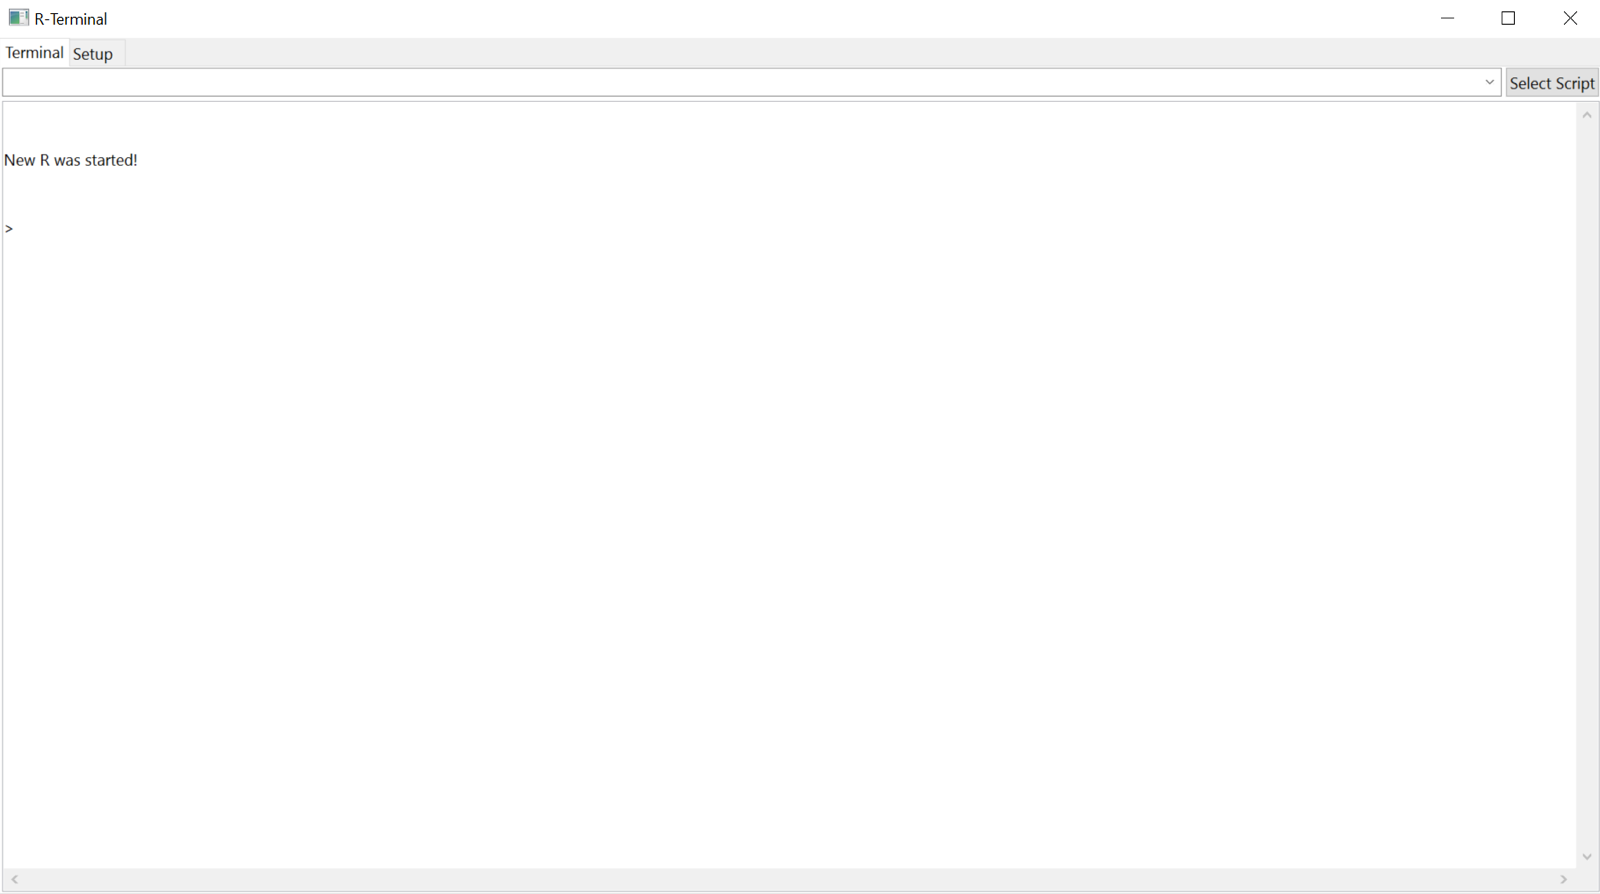
\includegraphics[width=0.8\textwidth]{Bilder/rterminalwindows}
\caption{R-Terminal: \textit{Terminal} unter Windows 10 Education (Version 1511)}
\label{rterminalwindows}
\end{figure}

\begin{figure}[htpb]
\centering
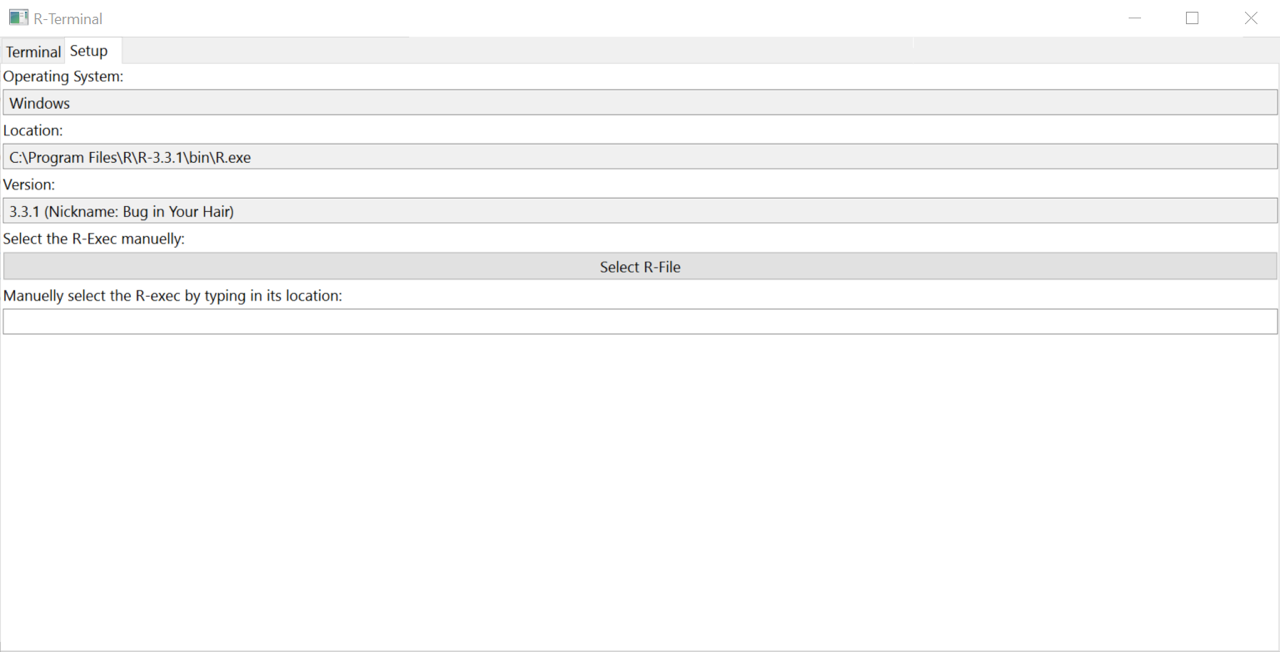
\includegraphics[width=0.8\textwidth]{Bilder/R-TerminalWindows}
\caption{\textit{R-Terminal}: \textit{Setup} unter Windows 10 Education (Version 1511)}
\label{rterminalwindows}
\end{figure}

\begin{figure}[htpb]
\centering
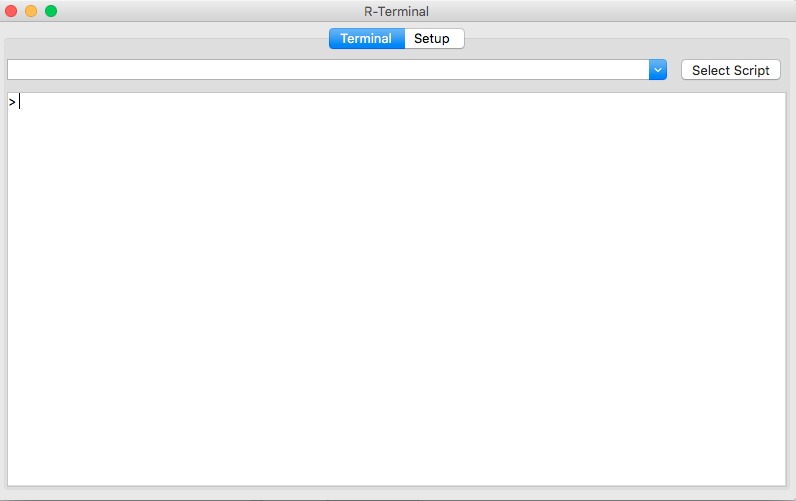
\includegraphics[width=0.8\textwidth]{Bilder/R-Terminal}
\caption{\textit{R-Terminal}: \textit{Terminal} unter OS X (Version 10.11.1)}
\label{rterminalmac}
\end{figure}

\begin{figure}[htpb]
\centering
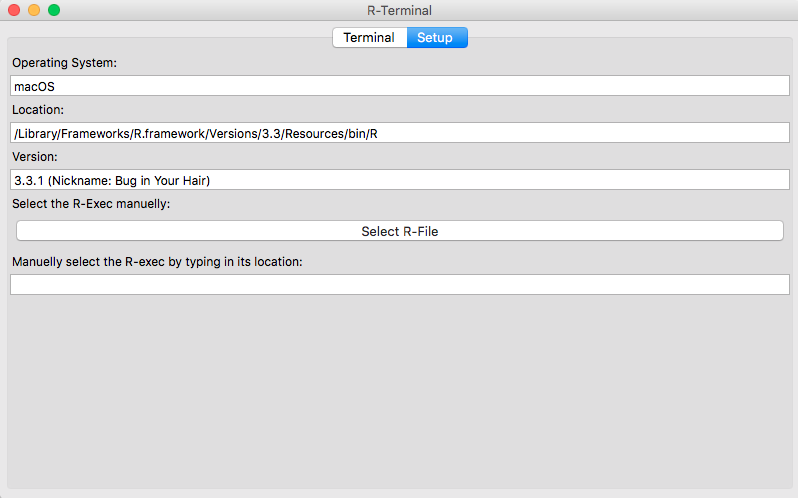
\includegraphics[width=0.8\textwidth]{Bilder/rterminalsetup}
\caption{\textit{R-Terminal}: \textit{Setup} unter OS X (Version 10.11.1)}
\label{macsetup}
\end{figure}
Diese wird für das Betriebssystem \textit{OS X} in Abbildung \ref{rterminalmac} dargestellt. Das Terminal verfügt über die zwei Tabs \textit{Terminal} und \textit{Setup} (S. \pageref{macsetup}). In Folgenden werden die beiden Tabs sowie deren Bedienung ausführlich erklärt.

\subsection{Setup} \label{Setup}
Unter \textit{Setup} wird entweder eine \textit{R}-Version auf dem Rechner gesucht und automatisch ausgeführt oder es wird vom Benutzer selber der Pfad zu der gewünschten \textit{R}-Version angegeben. 

Hierbei gibt das Feld unter \textit{Operating System} das Betriebssystem der benutzten Plattform an. Das Feld \textit{Location} gibt den Pfad an, unter dem die automatische Suche die ausführbare \textit{R}-Version gefunden hat. Konnte keine ausführbare R-Version gefunden werden, wird in dem Feld die Nachricht \textit{No valid R-exec found!} angezeigt. 

Das mit \textit{Version} betitelte Feld gibt die Version an, die die gefundene \textit{R}-Version hat. Wurde keine ausführbare \textit{R}-Version gefunden oder eine ungültige \textit{R}-Version angegeben, zeigt das Feld die Ausgabe \textit{No valid R-Version selected}an. 

Sind auf dem Rechner mehrere \textit{R}-Versionen vorhanden, von denen der Benutzer eine andere Version bevorzugt, als die durch die automatische Suche gefundene, gibt es die beiden unteren, im folgenden erläuterten Felder als Optionen. 

\textit{Select the R-Exec manually} öffnet eine Ordnerübersicht, durch die dann die zu der gewünschten \textit{R}-Version navigiert werden kann. Hierbei sollte beachtet werden, dass nicht der Pfad zu der \textit{R-GUI} angegeben werden sollte, welche oft zusammen mit dem \textit{R}-Executable installiert wird, sondern zu der ausführbaren \textit{R}-Datei.
  
Das letzte Feld \textit{Manually select the R-exec by typing in its location} gibt dem Benutzer die Möglichkeit, den bereits bekannten Dateipfad zur ausführbaren \textit{R}-Datei anzugeben. Hierbei sollte ein absoluter Dateipfad angegeben werden, der die ausführbare \textit{R}-Datei enthält (im Gegensatz dazu, nur den Ordner anzugeben, in dem die Datei liegt). 

Wird in \textit{Select the R-Exec manually} oder in \textit{Manually select the R-exec by typing in its location} eine ungültige \textit{R} Version oder ein ungültiger Dateipfad angegeben, wird unter \textit{Operating System} und \textit{Version} dieselbe Fehlermeldung angegeben, wie oben bei dem Fehlschlagen der automatischen Suche beschrieben. 

\subsection{Terminal} \label{Terminal}
Nachdem die gewünschte \textit{R}-Version gefunden wurde, kann diese nun unter dem Tab \textit{Terminal} bedient werden. Das Eingabefeld kann benutzt werden, um \textit{R}-kompatible Befehle auszuführen. Es werden bis zu 10 Befehle gespeichert. Diese können ausgewählt werden, indem auf den Pfeil auf der rechten Seite des Eingabefeldes geklickt wird. Dadurch öffnet sich ein Dropdown-Menü, aus dem der gewünschte Befehl ausgewählt werden kann. Dieser erscheint im Eingabefeld. Rechts neben dem Eingabefeld gibt es den Button \textit{Select Script}. Dieser Button öffnet bei Aktivierung eine Ordnerübersicht, aus der ein \textit{R}-Skript ausgewählt werden kann, welches dann ausgeführt wird. 


\chapter{Datenübertragung von ARX nach R} \label{NutzungArx}
Dieser Abschnitt beschreibt die wichtigsten \textit{R}-Befehle, die verwendet werden können um aus \textit{ARX} heraus mit dem vorgestellten Konzept Daten nach R zu transferieren.


\section{Datentypen und Skalenniveau}\label{Skalen}
In der medizinischen Statistik ist die Unterscheidung von den verschiedenen Stufen der Skalierbarkeit von großer Bedeutung. Für die Daten aus \textit{ARX} sind vor allem die Eigenschaften wichtig, die Patientenmerkmale besitzen. So können Merkmale in quantitative und qualitative Merkmale unterteilt werden \cite{skalenniveau}. Es ist kein Problem, quantitative Merkmale darzustellen, da diese einfach durch numerische Werte ausgedrückt werden können. Die Grunddatentypen sind wie folgt:

\begin{itemize}
\item \texttt{Numeric}
\item \texttt{Integer}
\item \texttt{Complex}
\item \texttt{Logic}
\end{itemize}

Wenn also eine Variable als Dezimalzahl ohne zusätzliche Bedingung deklariert wird, ist der Datentyp standardmäßig \texttt{numeric} (vgl. \ref{numericVar}).

\lstset{language=R}
\begin{lstlisting}[frame=single,caption={Deklarierung einer numerischen Variable x}]
> x = 13.4
\end{lstlisting}
\label{numericVar}

Will man explizit einen Integer als Variable initialisieren, sieht der Befehl aus wie in \ref{integerVar}. Es sollte zusätzlich beachtet werden, dass \texttt{TRUE} und \texttt{FALSE} in R jeweils die Ganzzahlwerte 1 und 0 besitzen. 

\lstset{language=R}
\begin{lstlisting}[frame=single,caption={Deklarierung einer ganzzahligen Variable y}]
> y = as.integer(4.5)
> y 	# gibt y als Wert aus 
[1] 4
\end{lstlisting}
\label{integerVar}

Um eine Variable mit dem Typ \texttt{complex} zu initialisieren, wird der imaginäre Teil der komplexen Zahl bei der Initialisierung angegeben. Ein Beispiel dazu ist in \ref{complexVar} zu sehen.

\lstset{language=R}
\begin{lstlisting}[frame=single,caption={Deklarierung einer komplexen Variable z}]
> z = 2 + 5i
\end{lstlisting}
\label{complexVar}

Die Datentypen können jeweils durch den Befehl \texttt{class()} abgefragt werden. Die Ausgaben sind in \ref{class} zu sehen. 

\lstset{language=R}
\begin{lstlisting}[frame=single,caption={Abfrage des Datentypen}]
> class(x)
"numeric"
> class(y)
"integer"
> class(z)
"complex"
\end{lstlisting}
\label{class}

Nachdem nun die quantitativen Merkmale dargestellt werden können, stellt sich die Frage nach der Darstellung der qualitativen Merkmalen. 

Die qualitativen Merkmale werden in nominalskalierte und ordinalskalierte Merkmale unterteilt. Ordinallskalierte Merkmale haben eine vorbestimmte Ordnung untereinander, die nicht zwangsläufig eine lineare Beziehung zueinander haben müssen. Nominalskalierte Merkmale sind hingegen eindeutige Kategorien, die untereinander keine Ordnung haben. 

Die einfachste Möglichkeit, einer Variable ein qualitatives Merkmal zuzuordnen, ist es als \texttt{character} zu definieren. Dies geschieht durch eine einfache Zuweisung wie in \ref{characterVar}.


\lstset{language=R}
\begin{lstlisting}[frame=single,caption={Deklarierung einer qualitativen Variable a}, float=htb]
> a = "verheiratet"     #nominalskaliertes Merkmal
> class(a)
"character"
> b = "befriedigend"	#ordinalskaliertes Merkmal
> class(b)
"character"
\end{lstlisting}
\label{characterVar}

Dies ist allerdings keine optimale Lösung, da hierdurch keine eindeutige, abgegrenzte Kategorisierung der Variablen stattfindet. Im Falle der ordinalskalierten Variablen kann auch keine Ordnung unter den Variablen festgelegt werden. Möchte man ein Histogramm erstellen, was bei qualitativen Merkmalen sehr wahrscheinlich ist, werden die Strings nicht als Instanz eines Attributs gezählt, sondern einfach nur als Strings. Um also eine bessere Darstellung für qualitative Merkmale zu erreichen, gibt es sogenannte \texttt{factor variables}. Hierbei kann ein Vektor aus Integers erstellt werden, wo jedem Integer ein \texttt{label} zugewiesen wird. Ein Beispiel dazu ist in \ref{factorVar} zu sehen. 

\lstset{language=R}
\begin{lstlisting}[frame=single,caption={Erstellung einer \texttt{factor variable}}, float=htb]
> v=c(0, 1, 1, 0, 1) #Vektorinitialisierung
> v
[1] 0 1 1 0 1		#Ausgabe von v
> einheiten=factor(v,labels=c("metrisch","imperial"))
> einheiten 
[1] metrisch imperial imperial metrisch imperial
Levels: metrisch imperial
\end{lstlisting}
\label{factorVar}

Nun konnte den verschiedenen Werten im Vektor \texttt{v} ein \texttt{label} zugeordnet werden. Zu beachten ist hierbei, dass der \texttt{labels}-Vektor entweder 1 oder genauso viele Elemente beinhaltet, wie verschiedene Werte im Basisvektor \texttt{v} enthalten sind. Die Zeile \textit{Levels} gibt die Ordnung der Merkmale an. Hierbei wurde \textit{metrisch} auf den ersten Wert gesetzt, der im Vektor \texttt{v} vorkommt, \textit{imperial} auf den ersten Wert, der von \textit{metrisch} verschieden ist. Dadurch konnte eine eindeutige Ordnung unter den Merkmalen festgelegt werden, nämlich \textit{imperial} $>$ \textit{metrisch}. Dies ist für dieses einfache Beispiel allerdings sinnlos, da keine Ordnung unter dem metrischen und imperialen System besteht.  Natürlich ist es ebenfalls möglich, eine \texttt{factor variable} direkt anhand von Strings zu erstellen, s. \ref{strFactorVar}.

\lstset{language=R}
\begin{lstlisting}[frame=single,caption={Erstellung einer \texttt{factor Variable} mit Strings}]
> w=c("sehr gut", "gut", "gut", "ausreichend", 
"mangelhaft", "sehr gut", "befriedigend", 
"gut", "ausreichend", "gut", "befriedigend")
> factor(w)
 [1] sehr gut gut          gut ausreichend mangelhaft  
 [6] sehr gut befriedigend gut ausreichend gut         
[11] befriedigend
Levels:ausreichend befriedigend gut mangelhaft sehr gut
\end{lstlisting}
\label{strFactorVar}

Es wurden mit der \texttt{factor}-Funktion direkt \textit{Levels} erstellt, die allerdings nicht die gewünschte Ordnung haben, die wir von den Schulnoten im Beispiel erwartet hätten. Dies ist aufgrund der automatischen alphabetischen Sortierung der Levels. Für eine selbst erstellte Ordnung, siehe \textit{R}-Befehl \ref{factorVar}. 

\lstset{language=R}
\begin{lstlisting}[frame=single,caption={Ordnen einer selbsterstellten \texttt{factor Variable}}]
> noten = ordered(w, levels=("sehr gut", "gut", 
"befriedigend", "ausreichend", "mangelhaft"))
> noten
 [1] sehr gut gut          gut ausreichend  mangelhaft  
 [6] sehr gut befriedigend gut ausreichend  gut         
[11] befriedigend
Levels: sehr gut < gut < befriedigend 
< ausreichend < mangelhaft
\end{lstlisting}
\label{factorVar}

Hier sieht man nun auch eine eindeutige Ordnung unter den Notenstufen \cite{factorVariables}. Die Bedeutung der \texttt{factor}-Funktion in Anwendung auf Vektoren wird im folgenden Abschnitt erklärt. 

Zusätzlich gibt es das \textit{R}-Package \texttt{memisc}. Diese Erweiterung weist Objekten, die ein \texttt{item} sind, ein \texttt{level of measurement} (Skalenniveau) zu, das entweder ein \textit{ordinal, nominal, interval} oder \textit{ratio} ist. Je nach dem Skalenniveau wird das \texttt{item} in einen \texttt{factor} (\textit{nominal}), einen geordneten Vector (\textit{ordinal}) oder einen numerischen Vektor (\textit{interval und} \textit{ratio}) konvertiert. 

\section{Tabellen} \label{tabellen}

In \textit{R} wird üblicherweise zur Darstellung von Tabellen ein \texttt{data.frame} verwendet. 

Ein \texttt{data.frame} ist eine Liste von Vektoren, welches mit dem Befehl \texttt{data.frame()} erstellt werden kann (s. \ref{dataframe}) \cite{dataFrame}.

\lstset{language=R}
\begin{lstlisting}[frame=single,caption={\texttt{data.frame} aus 3 Vektoren}]
> v1 = c(1,2,3)
> v2 = c("a","b","c")
> v3 = c(FALSE, FALSE, TRUE)
> frame = data.frame(v1, v2, v3)
> frame
  v1 v2    v3
1  1  a FALSE
2  2  b FALSE
3  3  c  TRUE
> names(frame) = c("Zahl", "Buchstabe", "Bool")
> frame
  Zahl Buchstabe  Bool
1    1         a FALSE
2    2         b FALSE
3    3         c  TRUE

\end{lstlisting}
\label{dataframe}

Mithilfe der in Abschnitt \ref{Skalen} beschriebenen Funktionen können die Spaltenvektoren in das gewünschte Skalenniveau konvertiert werden.
 
Für die Nutzung von \textit{ARX} mit dem \textit{R-Terminal} können die bereits vorhandenen Daten auch aus \textit{ARX} als CSVs eingeladen werden. 
Diese werden in ein \texttt{data.frame} gelesen, wie in Beispiel \ref{readTable} gezeigt.

\lstset{language=R}
\begin{lstlisting}[frame=single,caption={Einlesen einer Tabelle}]
frame=read.csv(file="c:/test.csv",header=TRUE,sep=",")
\end{lstlisting}
\label{readTable}

Die hier verwendeten Argumente sind einmal das \texttt{file}, der \texttt{header} und \texttt{sep}. \texttt{file} gibt den Dateipfad zu der CSV-Datei an. Hierbei kann auch ein Pfad angegeben werden, der relativ zum Arbeitsordner ist. \texttt{header} gibt an, ob in der Datei die erste Zeile ein Header ist, in dem die Namen der Spaltenattribute stehen, oder ob keine Namen für die Spalten vorhanden sind und in der ersten Zeile direkt der Inhalt der Tabelle beginnt. \texttt{sep} gibt den Character an, durch den die Spalten getrennt sind. 

Möchte man ein \texttt{data.frame} erweitern, z.B. durch eine neue Zeile oder eine neue Spalte, gibt es dafür die Funktionen \texttt{rbind} und \texttt{cbind}. Die Funktionen sind anzuwenden wie in \ref{readTable} vorgestellt. 

\lstset{language=R}
\begin{lstlisting}[frame=single,caption={\texttt{rbind} und \texttt{cbind}}, float=htb]
#Hierbei auf die gleichen Spaltennamen achten
> frame2 = data.frame(Zahl=4,Buchstabe="d",Bool=TRUE)
#frame aus data.frame
> newframe=rbind(frame, frame2)		
> newframe
  Zahl Buchstabe  Bool
1    1         a FALSE
2    2         b FALSE
3    3         c  TRUE
4    4         d  TRUE
######################
#Hier geht auch ein Vektor
> Nummer = c(4, 3, 2, 1)
> cbind(newframe, Nummer)
  Zahl Buchstabe  Bool Nummer
1    1         a FALSE  4
2    2         b FALSE  3
3    3         c  TRUE  2
4    4         d  TRUE  1

\end{lstlisting}
\label{readTable}

%Bei der Verwendung von \texttt{data.frame} sollte beachtet werden, dass zwar nützliche Funktionen verwendet werden können, sich das \texttt{data.frame} ausschließlich 
%insert Erklärung zu data.table und data.matrix?

\section*{Implementierung in zukünftigen Arbeiten}

Die in diesem Kapitel vorgestellten Befehle zur Übertragung von Tabellen aus \textit{ARX} nach \textit{R} wurden noch nicht im \textit{RTerminal} implementiert, sondern dienen als Vorarbeit für die Implementierung in zukünftigen Arbeiten.
%Um Tabellen aus \textit{ARX} in \textit{R} mithilfe des \textit{RTerminal} zu bearbeiten, müssen diese aus \textit{ARX} als CSV-Datei exportiert und anschließend, wie in diesem Kapitel beschrieben, eingelesen werden.

\chapter{Zukünftige Arbeiten}

Das \textit{R-Terminal}, welches im Rahmen dieser Arbeit erstellt wurde, setzt die Integration von \textit{R} in \textit{Java} um. 
Allerdings müssen anonymisierten Daten bisher noch manuell aus \textit{ARX} als Tabellen in CSV-Format exportiert werden und anschließend durch das \textit{RTerminal} an den \textit{R}-Prozess übergeben werden. Dieser manuelle Import sowie die Anpassung der Datenrepräsentation der Tabellen in \textit{R} wird in Kapitel \ref{tabellen} beschrieben.

Der bisherige Entwicklungsstand bietet aufgrund der nicht vorhandenen automatisierten Übertragung von Daten von \textit{ARX} nach \textit{R} noch keine vollständige Integration. Die im Rahmen dieses Projektes systematisch dokumentierten Befehle bieten aber eine solide Grundlage für zukünftige Projekte, in denen diese Funktionalität umgesetzt werden soll.


%----------------------------------------------------------------------------------------
%	BIBLIOGRAPHY
%----------------------------------------------------------------------------------------

%\bibliographystyle{unsrt}

%\bibliography{sample}
\begin{thebibliography}{9} %Das ist nur ein Beispiel, 1 und 2 sind im dummy text oben eingebunden 
%\bibitem{latexcompanion} 
%Michel Goossens, Frank Mittelbach, and Alexander Samarin. 
%\textit{The \LaTeX\ Companion}. 
%Addison-Wesley, Reading, Massachusetts, 1993.
 
%\bibitem{einstein} 
%Albert Einstein. 
%\textit{Zur Elektrodynamik bewegter K{\"o}rper}. (German) 
%[\textit{On the electrodynamics of moving bodies}]. 
%Annalen der Physik, 322(10):891–921, 1905.

\bibitem{license}
The Apache Software Foundation. \\
\texttt{https://www.apache.org/licenses/GPL-compatibility.html}, Januar 2016
\bibitem{sdc}
The R Foundation.\\
\texttt{https://cran.r-project.org/web/packages/sdcMicro/index.html}, Februar 2016
\bibitem{skalenniveau}
Institut Institut für Biometrie und Klinische Epidemiologie,\\
Universitätsklinikum Benjamin Franklin \\
\texttt{https://biometrie.charite.de/fileadmin/user\_upload/microsites/m\_cc04/ biometrie/Q1/SkriptQ1.pdf}, Januar 2016
\bibitem{dataFrame}
R Tutorial. An Introduction to Statistics, Chi Yau \\
\texttt{http://www.r-tutor.com/r-introduction/data-frame}, Januar 2016
\bibitem{rproject}
The R Foundation.\\
\texttt{https://www.r-project.org/about.html}, Januar 2016
\bibitem{eclipse}
The Eclipse Foundation. \\
\texttt{https://www.eclipse.org}, Januar 2016
\bibitem{swt}
The Eclipse Foundation. \\
\texttt{https://www.eclipse.org/swt/}, Januar 2016
\bibitem{java}
Oracle Corporation. \\
\texttt{https://www.java.com/de/}, Januar 2016
\bibitem{factorVariables}
UC Regenta. \\
\texttt{http://www.ats.ucla.edu/stat/r/modules/factor\_variables.html}, Januar 2016
\bibitem{processBuilder}
Oracle Corporation. \\
\texttt{https://docs.oracle.com/javase/7/docs/api/java/lang/ProcessBuilder.html}, Januar 2016
\bibitem{arx}
Fabian Prasser*, Florian Kohlmayer*. (*Equal contributors)\\
Putting Statistical Disclosure Control Into Practice: The ARX Data Anonymization Tool.\\\texttt{http://arx.deidentifier.org}, Januar 2016



\end{thebibliography}
%----------------------------------------------------------------------------------------

\end{document}